% !TEX root = main.tex

% COMPLETE

\chapter{Mining metagenomes for new protein functions: applied to plastic hydrolases}
\chaptermark{Mining metagenomes for new protein functions}
\label{chapter:metagenomes}

% \section*{Abbreviations}\label{abbreviations}
% \addcontentsline{toc}{section}{Abbreviations}

% \begin{table}[ht!]
%     \centering
%     \begin{tabular}{ll}
%         \toprule
%         \textbf{Abbreviation} & \textbf{Phrase} \\ \midrule
%         ABH & α/β hydrolase \\
%         EC & Enzyme Commission \\
%         GO & Gene Ontology \\
%         GOLD & Genomes OnLine Database \\
%         HMM & hidden Markov model \\
%         \emph{I. sakaiensis} & \emph{Ideonella sakaiensis} \\
%         LCC & leaf-branch compost cutinase \\
%         MAG & metagenome-assembled genome \\
%         MDA & multi-domain architecture \\
%         MHET & mono(2-hydroxyethyl) terephthalic acid \\
%         ORF & open reading frame \\
%         PET & polyethylene terephthalate \\
%         PMBD & Plastics Microbial Biodegradation Database \\
%         \bottomrule
%     \end{tabular}
% \end{table}

\section{Introduction}

\subsection{Metagenomics and metagenome-assembled genomes}

Metagenomics is the study of all genetic material in an environment (biome or microbiome) \cite{Sberro2019}. Metagenomics typically refers to the study of DNA, whereas, metatranscriptomics refers to RNA. Microbiomes contain a large number of unknown species that have not yet been cultured. It has been estimated \cite{Rinke2013} that only $1\%$ of microorganisms have been cultured---dubbed `the uncultured majority' \cite{Rappe2003}. Many of these species are likely to be eukaryotic \cite{Saary2019}, whether small or single-celled. Metagenome-assembled genomes (MAGs) are genomes (assemblies) that are recovered from metagenomes by co-assembly of metagenome sequences.

Recently, there has been a growing interest in metagenomics. A number of causes have contributed to this, including sequencing becoming cheaper and easier, improved databases to store metagenomes and metadata, and increasing maturity of bioinformatics tools to process metagenomes. This has allowed microbiomes to be investigated on unprecedented scales, for example to understand the distribution of species in humans \cite{Huttenhower2012}, the human gut \cite{Almeida2019,Forster2019}, the oceans \cite{Sunagawa2015,Sunagawa2020}, and distributions of phages across many of the Earth's ecosystems \cite{Al-Shayeb2020}. This has, in turn, bettered our understanding of the interactions between biomes, hosts and microbes, and improve our knowledge of how microbiomes impact host health. The human gut microbiome has been shown to be dominated by environmental factors, rather than host genetics \cite{Rothschild2018}. In other words, cohabiting individuals share microbiomes, whereas, family members who do not live together have different microbiomes. Furthermore, the gut microbiome has been linked to mental health, quality of life and depression, via the microbiota-gut-brain axis \cite{Valles-Colomer2019}.

Metagenomics can be divided up into three steps, outlined in the sections below.

\subsubsection{Sample collection}

Under the metagenomic paradigm, biomes are sampled to collect bulk genetic information, which is analysed \emph{in toto}. Rich metadata are collected alongside genetic material to contextualise results and allow different data sets (possibly collected from the same biome) to be integrated. Examples of metadata include: the type of biome from which samples were collected, such as the human gut, soil, or sea water; the date and location that samples were collected; sequencing platform, data analysis pipeline, and versions of software used; as well as many other esoteric information about particular biomes.

Once a biome has been sampled, a number of further steps are required to prepare the sample to be sequenced \cite{Bachmann2018,Franzosa2014}. Sample preparation protocols impact the reconstruction quality of metagenomes \cite{Bowers2015}, especially from low biomass biomes, such as skin and soil. Metagenomics studies suffer from large technical variation, which can obscure any meaningful biological variation \cite{Lozupone2013,Voigt2015,Solonenko2013}. When technical variations have been controlled for, biological variation has been identified both spatially and temporally \cite{Raes2008,Voigt2015}. Sample preparation methods contribute greatly to the technical variation. For example, methods of DNA extraction have a large effect on the results of metagenomics studies \cite{Costea2017,Kallies2019}. Library preparation steps prior to sequencing bias which fragments are sequenced \cite{Sato2019}. Efforts are afoot to standardise sample preparation, in order to reduce technical variation \cite{Costea2017}.

\subsubsection{Sequencing of samples}

Following extraction, genetic material is sequenced to determine the sequence of DNA or RNA. The choice of sequencing platform affects the results of metagenomics studies \cite{Solonenko2013,Sevim2019}. Typically, short read Illumina sequencing is performed \cite{Rodrigue2010}, which typically generates reads $<500$ nt. Conceptually, Illumina sequencing is similar to Sanger-type dideoxynucleotide sequencing, but uses fluorescent-labelled nucleosides. Initially, metagenomics was only conducted using amplicon sequencing, where genomic regions of interest were first amplified using libraries of primers before being sequenced. This strategy is cheaper than WGS but only regions that have been selectively amplified are sequenced. On the other hand, WGS is more suitable to metagenomics, where the content of metagenomes is not known \emph{a priori}, because bulk DNA is sequenced.

Recently, long-read Nanopore sequencing \cite{Deamer2016} using the MinION sequencer has been gaining in popularity---even being used by PuntSeq in my own backyard to study the metagenome of the river Cam in Cambridge \cite{Urban2020}. Compared to Illumina sequencing, MinIONs are small, portable, inexpensive and simple to operate \cite{Jain2016}, which has democratised sequencing and genomics. In Nanopore sequencing, a polymer is ratcheted through a protein nanopore, which disrupts the ionic current across the nanopore \cite{GEORGE1996}. Polymer sequences can be decoded from the characteristic patterns of currents across nanopores. Nanopore sequencing can even be used to sequence proteins in real-time \cite{Ouldali2020}. Unlike Illumina sequencing, megabase-long contigs can be sequenced in one go using Nanopore sequencing, without needing to be fragmented. The main drawback of the platform is the high error rate, between $5\%$ and $15\%$ \cite{Rang2018}. As the errors are uniformly distributed across the length of the sequence sequence, high coverage depth can mitigate errors. Multiple sources contribute to the error rate, including the simultaneous influence of multiple bases on the current across the pore \cite{Rang2018}. It is thought that between five and six adjacent bases (corresponding to $4^5$ or $4^6$ possible $k$-mers) contribute to the signal at each position in the sequence. Efforts are being made to reduce the error rate, including updates to the sequencing chemistry. Contributions of multiple adjacent bases and a low signal-to-noise ratio produce an enigmatic signal, but computational approaches are being developed to improve the base calling accuracy \cite{Rang2018,Wick2019}.

Short- and long-read sequencing work synergistically and can be applied in tandem, each alleviating the drawbacks of the other. A key motivation for this is hybrid assembly of reads into contigs \cite{Antipov2016}. On one hand, short-reads have high accuracy, but are hard to assemble into long contigs. On the other hand, long-reads have low accuracy, but can help to bridge gaps in assemblies to form longer contigs \cite{Overholt2019}.

\subsubsection{Analysis of samples}

Metagenomics produces large volumes of data, on an unprecedented scale for the biological sciences. Processing these data requires new methods, such as MetaSPAdes \cite{Nurk2017} for genome assembly, MMseqs2 \cite{Steinegger2017} for sequence searches and Linclust \cite{Steinegger2018} for sequence clustering. Performances of various metagenomics tools were compared in a rigorous assessment \cite{Sczyrba2017}. MGnify \cite{Mitchell2020} provide a turnkey analysis pipeline for metagenome sequencing reads (https://github.com/EBI-Metagenomics/pipeline-v5) written in Common Workflow Language \cite{Amstutz2016}. Users need only upload their raw reads to the European Nucleotide Archive \cite{Amid2020} to be processed by the MGnify pipeline. MGnify is also a key database for metagenomics data.

Samples are generally analysed in four steps, outlined below.

\begin{enumerate}
    \renewcommand{\theenumi}{\Roman{enumi}}%
    \item \textbf{Assembly of reads into contigs}

    Raw sequence reads are passed through quality control. If necessary, adapter sequences are trimmed. Then, cleaned up reads are assembled into contigs using an assembler, such as MetaSPAdes \cite{Nurk2017}. Modern assemblers typically split reads up into $k$-mers and construct a De Bruijn graph \cite{BRUIJN1946}, $G = (V,E)$. In the graph, vertices represent all ($k-1$)-mers, which are connected by an edge if one vertex is the $[1 : k-1]$ prefix of a $k$-mer and the other vertex is the $[2:k]$ suffix \cite{Myers1995,Compeau2011}. Contigs are assembled from $k$-mers by finding a Eulerian cycle---a cycle is a path that starts and ends at the same vertex---where each edge is visited once in $\mathcal{O}(|E|)$ time. This strategy was originally devised to answer the Seven Bridges of Königsberg problem, which asked whether a route through the town of Königsberg exists that crosses each of its seven bridges once and only once \cite{Euler}. Euler devised new methods to prove that this problem has no solution, thus instigating the field of graph theory. Older assembly strategies represented $k$-mers as vertices \cite{Compeau2011} and relied on finding a Hamiltonian cycle, where each vertex is visited once. However, finding Hamiltonian cycles is NP-complete \cite{Garey1979}---it is a special case of the travelling salesman problem, where the distance between adjacent $k$-mers is $1$, and the distance between all other pairs is $2$---so this approach is intractable on anything but small contigs.

    \item \textbf{Predicting open reading frames}

    Once contigs have been assembled, they are polished to remove errors and scaffolded by joining contigs together \cite{Lantz2018}. MGnify predicts open reading frames (ORFs) and proteins from assemblies using Prodigal \cite{Hyatt2010} and FragGeneScan \cite{Ismail2014}.

    \item \textbf{Producing metagenome-assembled genomes}

    Recently, there has been a growing interest in metagenome-assembled genomes (MAGs) \cite{Sharon2013a}. MAGs are recovered from metagenomes, from which many MAGs are assembled, that approximately represent the diversity of a given community. MAGs were pioneered in 2004 by recovering two complete genomes from a biofilm with low species diversity \cite{Tyson2004}. Restrictions on the maximum diversity of species in a microbiome have since been lifted \cite{Almeida2019,Forster2019,Parks2017} by longer read lengths, improved assemblers and better binning algorithms, which has allowed MAGs to be recovered from diverse communities \cite{Bowers2017}. Binning assigns contigs to a bin if it is likely they are from the same genome. Various properties are used to determine the likeliness, including GC content, tetra-nucleotide frequency and depth of sequencing coverage \cite{Bowers2017}. MetaBAT is a popular binning algorithm \cite{Kang2015}. Binning increases the ability to recover genomes of rare species with low abundance in communities \cite{Albertsen2013}. A Nextflow pipeline for recovering MAGs is available in nf-core \cite{Ewels2020} (https://github.com/nf-core/mag). MAGs are assigned to a taxonomic group using GTDB-Tk \cite{Chaumeil2019}.

    \item \textbf{Assessing the quality of metagenomes}

    Genome-quality, measured by completeness and contamination, can be assessed by checking for presence of universally-conserved genes in particular taxa. Examples of tools include CheckM \cite{Parks2015} for prokaryotes, EukCC for eukaryotes \cite{Saary2019}, and Busco for both \cite{Seppey2019}. Scores generated by these tools are complementary to classical genome metrics, such as N$50$ (length of the shortest contig at $50\%$ of the genome length) or L$50$ (number of contigs that make up $50\%$ of the genome length). Other scores, such as the minimum information about a metagenome-assembled genome (MIMAG) have been devised \cite{Bowers2017}.
\end{enumerate}

% \subsection{Applications of metagenomics}
%
% Completing the three metagenomics steps above are the necessary steps required to process metagenome data into a usable format to begin the biological analysis stage. Metagenomics has been applied in many different, varied ways. Below, we highlight two applications of metagenomics to characterise the human gut microbiome and the global ocean microbiome.
%
% \subsubsection{Case study: human gut microbiome}
%
% \subsubsection{Case study: Tara oceans}

\subsection{The α/β hydrolase domain}

\label{sec:intro-abh}

α/β hydrolases (ABHs) are hydrolases that contain an ABH domain (\ref{fig:abh_domain_structure}). The ABH domain fold was first described in 1992 by structural comparisons of proteins that were of very different phylogenetic origin and catalytic function \cite{Ollis1992}. These proteins, whilst not sharing common sequences or substrates, had a characteristic fold, consisting of an eight-stranded beta-sheet sandwiched between two planes of alpha-helices. A conserved catalytic triad, consisting of nucleophile---histidine---acid residues located on loops between the alpha-helices and beta-sheets, performs catalysis \cite{Ollis1992}. The triad is reminiscent of the prototypical catalytic triad of serine proteases \cite{Matthews1967}, but the residues are arranged in the mirror inverse---a prototypical example of convergent evolution. Whilst the positions of the catalytic triad's side-chains are exquisitely conserved, the rest of the sequence is not conserved, leading to great structural diversity of the non-core domain structure \cite{Dessailly2010}. As such, the CATH ABH domain superfamily contains 34 structurally similar groups ($5$\AA\ complete-linkage clusters), composed of a conserved ABH domain core, that is embelished with many non-conserved structural elements. One consequence of this is that the substrate-binding site is not conserved, permitting ABHs to catalyse multifarious substrates \cite{Suplatov2012,Mindrebo2016}. To show how functionally diverse the superfamily is, its members are annotated with \num{1277} unique Gene Ontology (GO) terms and $458$ unique Enzyme Commission (EC) terms. The family includes diversely important enzymes, such as acetylcholinesterase, lipase, thioesterase, and various types of peptidases \cite{Holmquist2005}. A number of proteins relevant to biotechnology and pharmaceuticals also contain ABH domains, including many plastic-degrading enzymes, introduced in \ref{sec:intro-PETase}. Rather remarkably, the same ABH can catalyse endopeptidyl hydrolysis and epoxide ring opening, using a single catalytic triad \cite{Zheng2016}.

\begin{figure}[!hbt]
    \centering
    \ifredact
        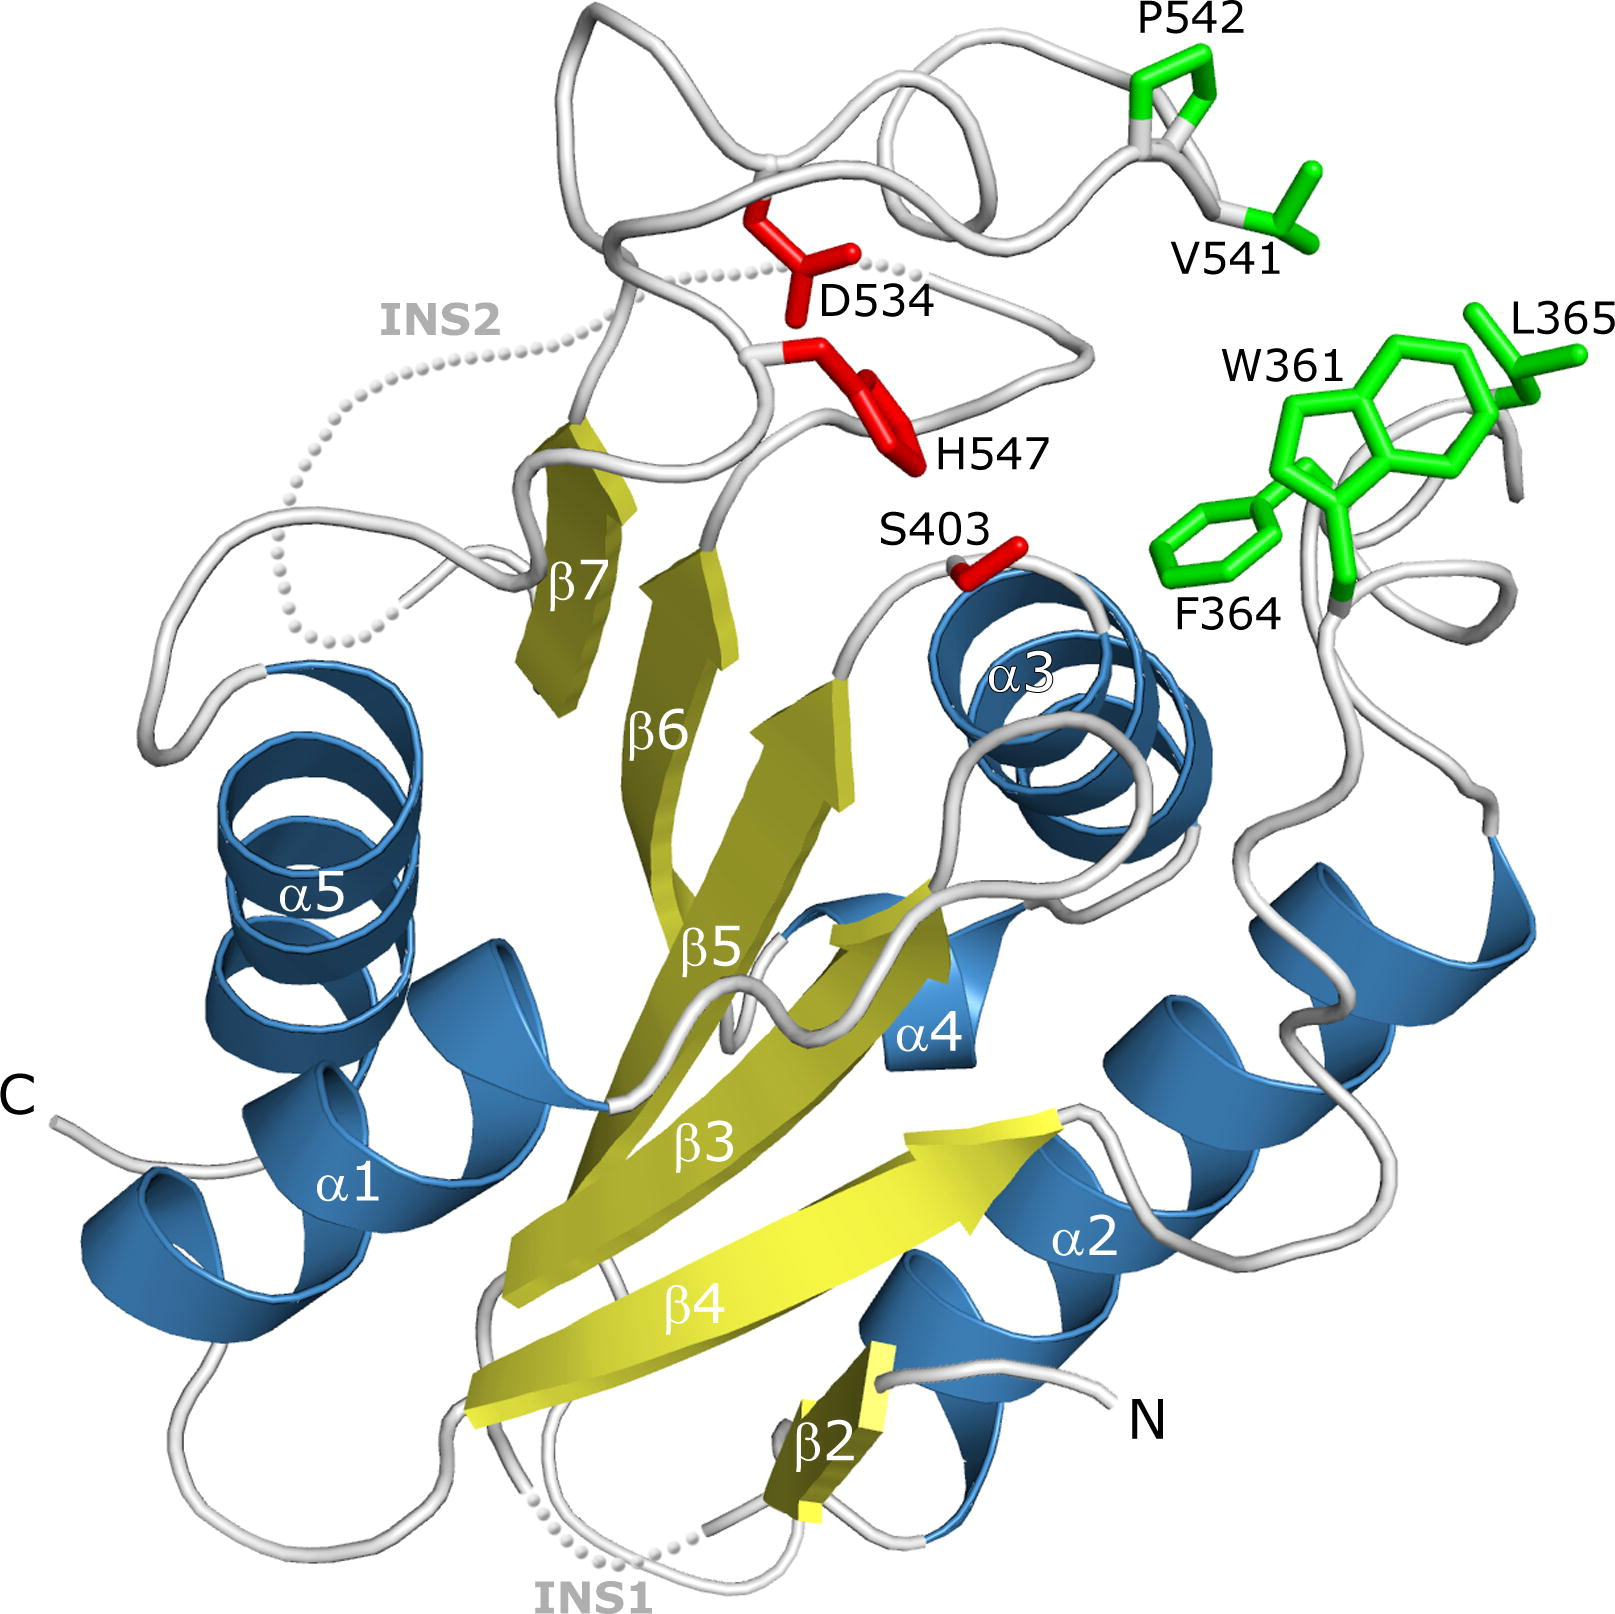
\includegraphics[draft=true]{./Chapter_metagenomes/abh_domain_structure}
    \else
        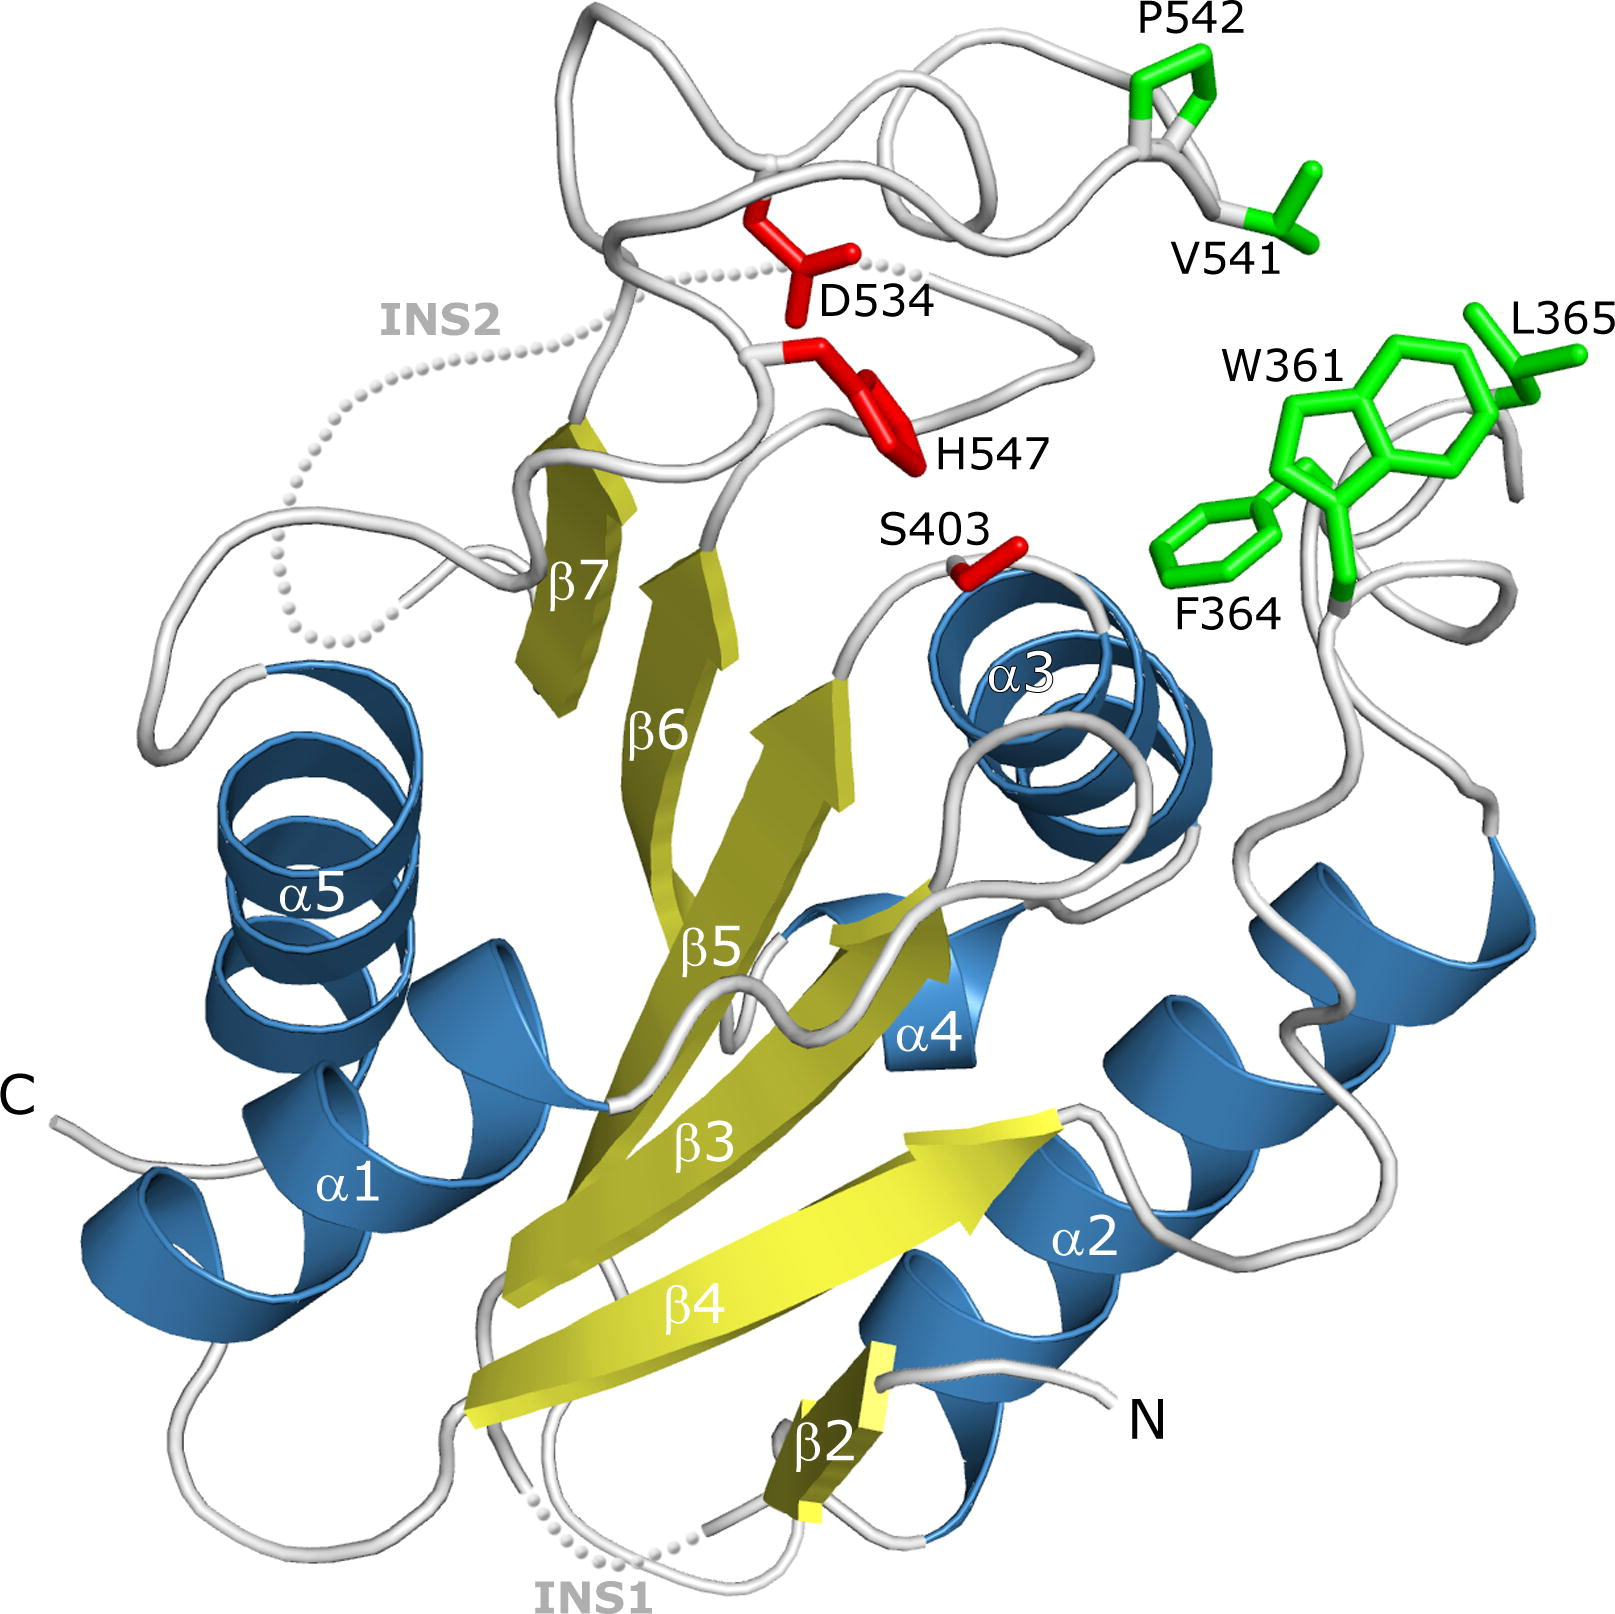
\includegraphics{./Chapter_metagenomes/abh_domain_structure}
    \fi
    \caption{%
        Structure of the α/β hydrolase domain fold.
        The $\beta$-sheet (yellow) is sandwiched between two planes of $\alpha$-helices (blue).
        The nucleophile—histidine—acid (S-H-D in this example) residues (red) are on loops.
        Figure from \cite{Lazniewski2011}.
        Structure of DUF2319 C-terminal catalytic domain from \emph{Mycobacterium tuberculosis} H37Rv.
        DUF2319 proteins lack $\beta$1 strand of the canonical fold.
    }
    \label{fig:abh_domain_structure}
\end{figure}

The ABH domain fold is represented in CATH as superfamily 3.40.50.1820. In the CATH hierarchy, the ABH domain is in the alpha beta class, three-layer alpha beta alpha sandwich architecture, and Rossmann fold \cite{Rao1973} topology. The ABH domain is one of the largest superfamilies in nature: Gene$3$D (v16) predicts \num{557283} ABH domains in UniProt \cite{Lewis2018,Bateman2019}. The ABH superfamily contains $377$ FunFams in CATH (v4.2).

\subsection{Polyethylene terephthalate (PET)}
\label{sec:intro-PET}

Plastics are polymers, whose building blocks are derived from crude oil and natural gas. Polyethylene terephthalate (PET) is the most abundant plastic in the world, from its extensive use in packaging and textiles \cite{Geyer2017}. PET is a polymer of mono(2-hydroxyethyl) terephthalic acid (MHET), which is produced from ethylene glycol and terephthalic acid. Used PET can be recycled by thermomechanical processes, but the resulting material has inferior properties, so a market for virgin PET persists \cite{Ragaert2017}. Globally, $311$ million tons of plastics are produced annually, of which PET accounts for $70$ million tons \cite{Bornscheuer2016}. Of concern, only $14\%$ of the plastic produced each year is collected for recycling \cite{Bornscheuer2016}. A devastating quantity of the remainder ends up polluting Earth, producing untold ecological \cite{Wilcox2015,Law2014,Rochman2018} and environmental \cite{Lebreton2018,Lacerda2019} damage. One poignant example is the not-so-great Great Pacific garbage patch in the North Pacific Ocean \cite{Lebreton2018}: \num{80000} tons of plastic in a vile tangle extending over $1.6$ million km$^2$---an area equivalent to the United Kingdom, France, Spain and Germany combined.

Two problems need to be solved to alleviate the impact of plastic on the environment. Firstly, bioremediation methods are required to clean up pollutants. Secondly, to reduce the demand for virgin plastics, recycling methods are required that can convert used plastic into high-quality materials. Both problems could be solved using plastic-degrading enzymes, or organisms.

\subsection{PET hydrolase enzymes}
\label{sec:intro-PETase}

Naturally-evolved enzymes are able to hydrolase PET. PET degradation has been shown in microbial communities \cite{Sharon2013} by bacterial hydrolases \cite{Muller2005} and cutinases \cite{Ronkvist2009,Vertommen2005}. All known PET hydrolases contain an ABH domain that is responsible for catalytic breakdown of PET. ABHs (\ref{sec:intro-abh}) are a large superfamily that have evolved a wide variety of functions and PET hydrolases are an exciting biotechnological application that could have a substantial positive impact on the environment.
In total, the Plastics Microbial Biodegradation Database (PMBD) lists $79$ proteins that are known to be involved in plastic degradation from $949$ microorganisms \cite{Gan2019}.
Furthermore PMBD predicted \num{8000} putative plastic-degrading proteins in UniProt.
In this chapter, we study the functional diversity of ABHs in metagenomes, focussing on sequences that are similar to a novel PET hydrolase, PETase.

\subsection{PETase}

In 2016, a new bacterial species was discovered that is able to metabolise PET as its only carbon source \cite{Yoshida2016,Bornscheuer2016}. \emph{Ideonella sakaiensis} (\emph{I. sakaiensis}) was isolated from outside a plastic recycling plant in Japan, living on PET bottles---an extreme, unnatural environment, with a high selection pressure to evolve PET metabolism. Two enzymes are responsible: PETase, which depolymerises PET into MHET, and MHETase, which breaks MHET down (\ref{fig:petase_mhetase}). The resulting ethylene glycol and terephthalic acid and metabolised by \emph{I. sakaiensis} to provide ATP.

A number of concerns \cite{Yang2016a} were voiced by Yang \emph{et al.} about the work presented by Yoshida \emph{et al.} \cite{Yoshida2016}. Firstly, Yang identifies that a low crystallinity PET ($1.9\%$) was used to test the efficiency of PETase. Typically, commercial PET bottles have \numrange{30}{40}$\%$ crystallinity. A cutinase from \emph{Fusarium solanipisi} that hydrolases PET was shown to have a non-linear decrease in PET hydrolysis efficiency as the crystallinity increased \cite{Vertommen2005}. Therefore, PETase was tested on a substrate that is not representative of how the enzyme will most likely be used in the wild. Secondly, Yoshida did not measure the mass of PET to show that it was broken down by \emph{I. sakaiensis}. Instead, they showed a gel permeation chromatogram and presented almost identical traces between a $22$ day PETase experiment and a $0$ day negative control. Yoshida argue that PET hydrolysis only occurred at the surface of the PET film, but Yang counter argue that breakdown of PET on the surface could be caused by the mechanical action (i.e. not enzymatic) of \emph{I. sakaiensis} on the surface of the film. However, Yoshida argue \cite{Yoshida2016a} that their intention was simply to present a microorganism that can grow on PET, and to identify the enzymes that permit this growth. They also argue that microbial degradation of PET had previously been confirmed \cite{Sharon2013}. In sum, \emph{I. sakaiensis} is able to grow on PET, using PETase, but PETase has not been shown to be able to efficiently hydrolyse the types of PET that are used prolifically in commercial situations.

\begin{figure}[!hbt]
    \centering
    \ifredact
        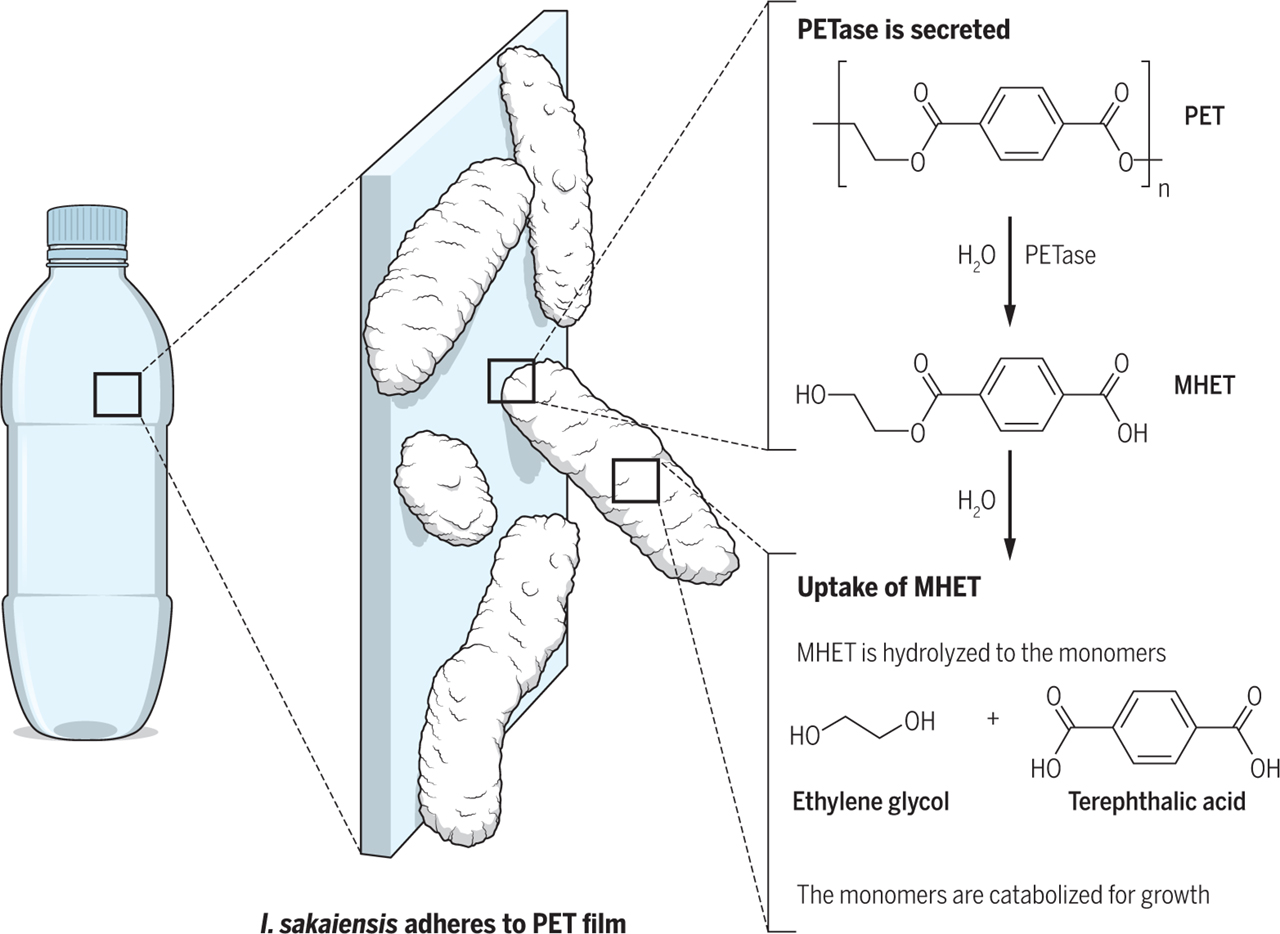
\includegraphics[draft=true]{./Chapter_metagenomes/petase_mhetase}
    \else
        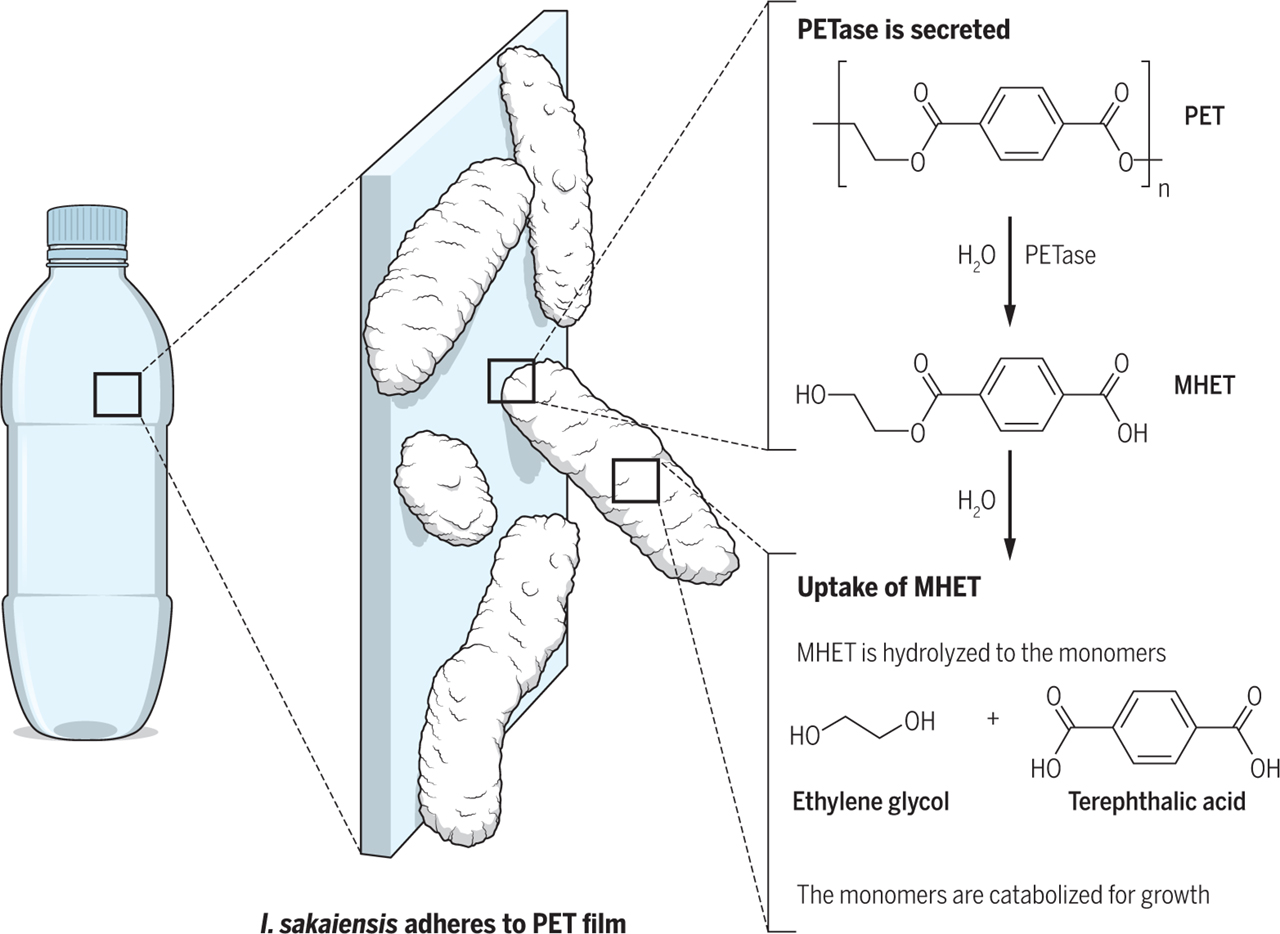
\includegraphics{./Chapter_metagenomes/petase_mhetase}
    \fi
    \caption{%
        Two enzymes are responsible for PET hydrolysis in \emph{I. sakaiensis}.
        PETase depolymerises PET into MHET, followed by MHETase, which breaks MHET down into ethylene glycol and terephthalic acid.
        Figure from \cite{Bornscheuer2016}.
    }
    \label{fig:petase_mhetase}
\end{figure}

Whilst PETase and MHETase are responsible for PET degradation \cite{Yoshida2016}, the exact mechanisms are unknown. Structural studies have proposed potential mechanisms \cite{Han2017,Joo2018,Austin2018,Palm2019}. Despite evolving in a PET-rich environment, PETase does not hydrolyse PET optimally \cite{Austin2018}. PETase was modified to narrow the substrate binding cleft, by introducing conserved amino acids that are found in the equivalent positions in cutinases, which improved PET degradation \cite{Austin2018}. But this improvement pales in comparison to leaf-branch compost cutinase (LCC) that degrades PET four orders of magnitude faster than PETase \cite{Tournier2020}. Disulfide bridges were engineered into LCC to make it more thermostable. Post-consumer PET waste was efficiently processed by LCC, with an estimated material cost of required protein at $4\%$ of the ton-price of virgin PET. As a tour de force, PET was then completely recycled using LCC, whereby the breakdown products of ethylene glycol and terephthalic acid, were used to re-form PET, demonstrating the potential for a circular economy \cite{Tournier2020}.

\subsection{Contributions}

The plastic bottle has transitioned from a modern miracle to an environmental scourge, within a generation. Enzymatic bioremediation and recycling of PET is a promising solution to this problem. PET hydrolases are an exciting class of natural enzymes that have recently evolved to degrade PET. Metagenomes are large, untapped reservoirs of novel functions.

In this chapter, we mine metagenomes for ABH domains that may degrade PET or other plastics. We analyse how metagenomic proteins from the MGnify database are distributed between the biomes. Using hidden Markov models (HMMs) of CATH superfamilies from Gene$3$D and FunFams, we identified \num{500000} ABH domains and \num{400000} FunFam domains in MGnify. ABH domains are signficantly enriched in engineered (non-natural) biomes. Metagenomes contain a wide diversity of ABH domains that share only limited overlap with known ABH domains in UniProt. Metagenomic ABH domains share higher sequence similarity with ABH domains from prokaryotes in UniProt, compared to ABH domains from eukaryotes. Many metagenomic ABHs are novel and rare, but those that are common in metagenomes are also found in UniProt. There is little evidence for the evolution of novel domains in metagenomic proteins that contain an ABH domain. Metagenomic ABH domains are distributed amongst the ABH FunFams in a completely different pattern to how ABH domains from UniProt are distributed.

Large sequence data sets are becoming increasingly common with the advent of large-scale genome sequencing and metagenomics. GARDENER, the current method for generating FunFams is unable to scale to data of this size. In this chapter, we also develop a new divide-and-conquer algorithm, FRAN, to generate FunFams on large sequence data sets. We rigorously benchmark the performance of FRAN and compare it to GARDENER.


\section{Methods}

\subsection{Data}

\subsubsection{MGnify}
\label{sec:mgnify-methods}

MGnify \cite{Mitchell2020} is a microbiome database. MGnify hosts metagenome sequences from microbiome studies. Typically, uploaded data sets are from shotgun metagenomics \cite{Quince2017}. MGnify assembles reads into contigs using metaSPAdes \cite{Nurk2017}, a De Bruijn graph assembler. With contigs longer than $500$ nucleotides in hand, RNA genes are predicted using Rfam \cite{Kalvari2018} and masked. ORFs are predicted in the remaining sequences using the prokaryotic gene callers Prodigal \cite{Hyatt2010} and FragGeneScan \cite{Ismail2014}. Prodigal is run first, followed by FragGeneScan for regions in which Prodigal does not predict any proteins. Protein sequences were clustered using Linclust at $90\%$ sequence identity with $90\%$ coverage of the centroid sequence (command line arguments \texttt{-\/-min-seq-id\ 0.90\ -c\ 0.9\ -\/-cov-mode\ 1}).

Metagenome studies are associated with metadata. One such datum is the biome from which the metagenome was sampled. Biomes are classified according to the Genomes OnLine Database (GOLD) \cite{Mukherjee2019} microbiome ontology, which is a directed acyclic graph that describes hierarchical relationships between biomes, akin to the Gene Ontology for function annotations. Whilst biome classification at the study level is mutually exclusive, it is not so at the protein sequence level because the same sequence can be found in multiple biomes. A selection of $13$ high-level ontological terms are associated with sequences (demarcated by *):

\begin{itemize}
\item Engineered*
\item Environmental
  \begin{itemize}
  \item Aquatic*
    \begin{itemize}
    \item Marine*
    \item Freshwater*
    \end{itemize}
  \item Soil*
    \begin{itemize}
    \item Clay*
    \item Shrubland*
    \end{itemize}
  \end{itemize}
\item Host-associated
  \begin{itemize}
  \item Plants*
  \item Human*
    \begin{itemize}
    \item Digestive system*
    \end{itemize}
  \item Human but not root
    \begin{itemize}
    \item Digestive system*
    \end{itemize}
  \item Animal*
  \end{itemize}
\item None of the above*
\end{itemize}

For reference, UniProt contains \num{181252700} sequences, comprised of \num{562253} Swiss-Prot sequences and \num{180690447} TrEMBL sequences (\ref{fig:n_seq}). Here, we used MGnify May 2019 release, which contains \num{1106951200} protein sequences (\ref{fig:n_seq}), generated from \num{12560} assemblies. A non-redundant set of \num{304820129} is available as S90 cluster representatives. From now on, we refer to the non-redundant sequences as `MGnify proteins'. MGnify contains vastly more sequences than UniProt, so is likely to contain novel functions yet to be discovered.

\begin{figure}[!hbt]
    \centering
    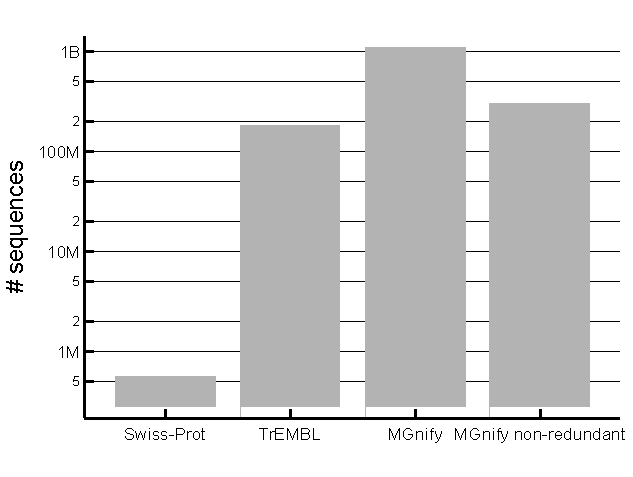
\includegraphics{./Chapter_metagenomes/n_seq}
    \caption{%
        Number of sequences in Swiss-Prot, TrEMBL and MGnify.
        MGnify non-redunant are S90 cluster representative sequences.
    }
    \label{fig:n_seq}
\end{figure}

\subsubsection{CATH, Gene$3$D and FunFams}

CATH, Gene$3$D and FunFams were introduced in \ref{sec:intro-cath,sec:intro-gene3d,sec:intro-funfam}. CATH \cite{Sillitoe2019} v4.2 and Gene$3$D \cite{Lewis2018} v16 were used. Superfamily HMMs in Gene$3$D v16 were generated using UniProt \cite{Bateman2019} August 2017 release. Gene$3$D contains models for \num{6119} superfamilies, represented by \num{65014} HMMs trained on multiple sequence alignments of S95 sequence identity clusters. ABH domain sequences predicted by Gene$3$D from UniProt August 2017 release were used.

\subsection{Software}

\subsubsection{Containers}

Singularity \cite{Kurtzer2017} v2.6.0 was used to run Singularity and Docker containers. Docker (https://www.docker.com) images were downloaded from Docker Hub (https://hub.docker.com) and BioContainers \cite{DaVeigaLeprevost2017}.

\subsubsection{HMMER}

HMMs and HMMER were introduced in \ref{intro-hmms}. HMMER \cite{Mistry2013} v3.2.1 was used from the Docker image ``biocontainers/hmmer:v3.2.1dfsg-1-deb\_cv1''.

\subsubsection{Linclust}

Linclust \cite{Steinegger2018} is a fast, greedy, single-linkage sequence clustering method in MMseqs2 \cite{Steinegger2017}. Due to some clever tricks, Linclust's runtime scales linearly with the number of sequences, independently of the number of clusters. First, Linclust performs an approximate and inexpensive clustering by assigning each sequence to multiple sets, or canopies \cite{McCallum2000}. Canopy clustering approaches improve time complexities by applying exact but expensive clustering methods to each canopy independently. Linclust uses sequence MinHashing \cite{Broder1998,Broder1997,Buhler2001,Ondov2016,Ren2018} to generate canopies. $p$ different hash functions are used to select the $p$ $k$-mers from each sequence with the lowest hash value. Here, we used $p = 21$. Sequences that share a $k$-mer are assigned to the same canopy. The longest sequence in each canopy is selected as the centroid sequence. Edges are added between centroids and the sequences in the canopy to form an initial single-linkage clustering. Expensive comparisons, such as sequence alignment, are only performed between $\le pn$ connected sequence pairs. $\mathcal{O}(pn)$ runtime complexity is achieved where $p << n$, compared with $\mathcal{O}(n^2)$ for all-against-all comparison. Finally, edges are removed between sequence pairs if one or more clustering criteria, such as the sequence identity threshold, are not met.

Linclust v10 was used from the Docker image ``soedinglab/mmseqs2:version-10''. Sequences were clustered at different sequence identity thresholds and coverage of centroid sequences, typically $30\%$, $50\%$, $70\%$ or $90\%$, (command line arguments: \texttt{-\/-min-seq-id\ \textless{}X\textgreater{}\ -\/-c\ \textless{}X\textgreater{}\ -\/-cov-mode\ 1}, where \texttt{X} is some percentage, provided as a fraction).

\subsubsection{cath-resolve-hits}

cath-resolve-hits was introduced in \ref{sec:intro-gene3d}. cath-resolve-hits \cite{Lewis2019} v0.16.2 was used to resolve domain boundaries in multi-domain architectures (MDAs). Different parameters were used depending on the context, so these are defined in the protocols. cath-resolve-hits was used from the Docker image ``harryscholes/cath-resolve-hits:0.16.2''.

\subsubsection{Nextflow}

Nextflow \cite{DITommaso2017} (v19.07.0.5106) was used to write and execute reproducible pipelines. Nextflow introduces a number of useful features for deploying pipelines, particularly in high-performance computing cluster environments. Nextflow pipelines are constructed from building blocks of `processes', arranged in linear or branched topologies. Each process contains a set of inputs, a script that processes the inputs, and a set of outputs. The script can be in any language, be it Bash, Julia or Python. Parallelism can be easily introduced by splitting inputs into chunks, to be processed separately. Processes only request their required CPU and memory resources from cluster queue managers. To achieve true portability, each process can be executed in a container (Docker and Singularity are supported), which can be automatically pulled from various container repositories. Intermediate results are cached, which allows pipelines to be resumed and updated without repeating a lot of computation. Many expert-written pipelines are available from nf-core \cite{Ewels2020}, a community effort to provide complex bioinformatics pipelines to users, requiring little (computational) domain-specific knowledge. In sum, Nextflow is one of many new tools, which make it easy to write and execute reliable and reproducible pipelines.

Where appropriate, pipelines described in this work are implemented in Nextflow. These pipelines are designed to be portable and reproducible. For example, input data are automatically downloaded where possible, processes are executed in Singularity containers, and data are processed in parallel for speed.

\subsection{Data analysis}

Data analyses were performed in Julia v1.3 \cite{Bezanson2012} using packages BioAlignments v2.0.0, BioSequences v2.0.1, CodecZlib v0.7.0, Combinatorics v1.0.0, CSV v0.6.1, DataFrames v0.20.2, DataStructures v0.17.11, FASTX v1.1.1, Formatting v0.4.1, GLM v1.3.9, HTTP v0.8.13, HypothesisTests v0.9.2, JSON v0.21.0, JSON2 v0.3.1, KernelDensity v0.5.1, Plots v1.0.5, StatsPlots v0.14.4, TranscodingStreams v0.9.5 and Unmarshal v0.3.1. Custom library code is released as CATHBase.jl \cite{Scholes2020}, which is available from https://github.com/harryscholes/CATHBase.jl.

\subsection{Finding domains in protein sequences}

In this context, we define a domain as a region of a protein sequence that has a significant hit to an HMM. The following protocol can be used to find domains in a database of protein sequences:

\begin{enumerate}
\def\labelenumi{\arabic{enumi}.}
\item Search the sequence database using a library of domain HMMs
\item For each protein:
  \begin{enumerate}
    \def\labelenumii{\roman{enumii}.}
    \item Resolve the MDA (optional)
    \item Extract domains
  \end{enumerate}
\end{enumerate}

This is a generic and flexible protocol to find domains in protein sequences. Below, we set out specific protocols that we used in this study to find CATH superfamily and FunFam domains in the MGnify protein database.

\subsubsection{Predicting CATH superfamily domains in protein sequences}
\label{sec:find_superfamily_domains}

CATH superfamily domains were predicted in protein sequences using \ref{algo:predict-superfamily-domains}. The MGnify protein database was searched using the Gene$3$D HMM library using hmmsearch from HMMER3 \cite{Mistry2013}. Hits were called using a threshold of E $< 0.001$ (command line arguments \texttt{-\/-domE\ 0.001\ -\/-incdomE\ 0.001}). It is often expedient to split the sequence database into manageable chunks, which can be searched independently and in parallel. For E-values to be calculated correctly, the size of the entire database must be provided to the \texttt{-Z} command line argument.

\begin{algorithm}[hbt!]
    \caption{%
        Predict CATH superfamily domains in protein sequences.
    }
    \label{algo:predict-superfamily-domains}
    \begin{algorithmic}[1]
        \Procedure{}{}
        \State scan sequences against the Gene$3$D HMM library
        \State resolve MDAs using cath-resolve-hits
        \State extract superfamily domains of interest from the resolved MDA coordinates
        \EndProcedure
    \end{algorithmic}
\end{algorithm}

cath-resolve-hits was used to resolve MDAs (command line arguments \texttt{-\/-min-dc-hmm-coverage=80\ -\/-worst-permissible-bitscore=25}). CATH superfamily IDs were assigned using the \texttt{assign\_cath\_superfamilies.py} Python script provided with Gene$3$D. If all domains were continuous, this process would be trivial, however, this is not the case and discontinuous domains complicate the process. Discontinuous HMMs are made up of multiple HMMs that model the separate continuous sequences. It is trivial to assign the MDA of a protein containing all continuous domains. For proteins that contain discontinuous domains, there is no correct way to assign the MDA string. Here, for a domain $D$ in protein $P$, we calculated its centre of mass $\mathbf{R}$ by
\[ \mathbf{R}(D|P) = \frac{\sum D_i}{\sum P_j} \]
for all $i$ residue numbers in $D$ and all $j$ residue numbers in $P$. MDAs were assigned by sorting domains according to their centre of mass.

ABH domain sequences were extracted from full-length sequences using the resolved start and stop positions of continuous domains and the concatenated sequence of discontinuous domains from the myriad start and stop positions.

\subsubsection{Predicting CATH superfamily domains in large sequence data sets}
\label{sec:find_superfamily_domains_in_large_dbs}

\begin{algorithm}[hbt!]
    \caption{%
        Predict CATH superfamily domains in large sequence data sets.
    }
    \label{algo:predict-superfamily-domains-large}
    \begin{algorithmic}[1]
        \Procedure{}{}
        \State scan sequences against a subset of the Gene$3$D HMM library
        \State create a subset of the sequences with a hit to one of the HMMs
        \State \ref{algo:predict-superfamily-domains} continues from Line 1
        \EndProcedure
    \end{algorithmic}
\end{algorithm}

In actuality, we used a modified version of \ref{algo:predict-superfamily-domains} to search for superfamily domains in the $300$ million MGnify proteins (\ref{algo:predict-superfamily-domains-large}). To reduce the amount of computation, we added additional steps. These steps are only appropriate if searching for a subset of domains.

First, the sequence database was searched using a subset of models. In this case, the MGnify proteins were searched using the Gene$3$D HMMs from the ABH superfamily and the same settings as \ref{sec:find_superfamily_domains}. Second, the sequences that have hits to the subset of models are extracted to create a derivative database that is likely to be much smaller than the original database. The derivative database is used as input to the protocol in \ref{sec:find_superfamily_domains}. This modified protocol is implemented as a Nextflow pipeline.


\subsubsection{Predicting FunFam domains in protein sequences}

FunFam domains were identified in sequences that contain ABH superfamily domains from \ref{sec:find_superfamily_domains_in_large_dbs} using \ref{algo:predict-funfam-domains}. These sequences were scanned against the FunFam HMM library using HMMER. The per FunFam inclusion threshold was used (command line options \texttt{-\/-cut\_tc}). MDAs were resolved using cath-resolve-hits (command line options \texttt{-\/-min-dc-hmm-coverage=80\ -\/-worst-permissible-bitscore=25\ -\/-long-domains-preference=2}). This protocol is also implemented as a Nextflow pipeline.

\begin{algorithm}[hbt!]
    \caption{%
        Predict FunFam domains in protein sequences.
    }
    \label{algo:predict-funfam-domains}
    \begin{algorithmic}[1]
        \Procedure{}{}
        \State scan sequences against FunFam HMMs
        \State resolve MDAs using cath-resolve-hits
        \State extract FunFam domains of interest from the resolved MDA coordinates
        \EndProcedure
    \end{algorithmic}
\end{algorithm}

\subsection{Protein sequence clustering}
\label{sec:clustering}

ABH domains from full-length MGnify sequences and UniProt were pooled to create a combined ABH domain data set. These sequences were clustered into single-linkage clusters using Linclust at $30\%$, $50\%$, $70\%$ and $90\%$ sequence identity and coverage of the cluster centroid sequence, implemented as a Nextflow pipeline.

\subsection{Kingdom-level taxonomy of UniProt ABH domains that cluster with MGnify ABH domains}

Mixed clusters, composed of ABH domains from MGnify and UniProt, from clustering at S30, S50, S70 and S90 (\ref{sec:clustering}) were used. The kingdom-level taxonomy of UniProt sequences in mixed clusters were downloaded using the Proteins API \cite{Nightingale2017}.


\subsection{Identifying whether novel domains have evolved in metagenomes}
\label{sec:intro-novel-domain}

C- and N-terminal regions and inter-domain regions of sequence may contain novel domains that evolved in metagnomes. To test the evidence for novel domain evolution, terminal and inter-domain sequence lengths were calculated from Gene$3$D hits (\ref{sec:find_superfamily_domains_in_large_dbs}). Inter-domain regions are defined as contiguous regions of sequence that do not have a significant match to any Gene$3$D HMM in the protein's MDA. Full-length proteins whose MDAs only contain continuous domains and do not contain discontinuous domains were considered. Single-domain proteins have two terminal regions, whereas, multi-domain proteins can also have inter-domain sequences between each pair of adjacent domains. Examples are shown below for domains (\texttt{@}) and terminal and inter-domain regions (\texttt{-}).

\noindent \textbf{i. Single-domain protein:}

\begin{figure}[H]
\begin{verbatim}
              -----@@@@@@@-----
    Terminal:   1           2
\end{verbatim}
\end{figure}

\noindent \textbf{ii. Multi-domain protein:}

\begin{figure}[H]
\begin{verbatim}
              -----@@@@@@@---@@@@@@@---@@@@@@@-----
    Terminal:   1                               4
Inter-domain:              2         3
\end{verbatim}
\end{figure}


\subsection{Identifying redundant domain sequences}

Full-length sequences were aligned pairwise by the banded Needleman-Wunsch algorithm \cite{Needleman1970} for global sequence alignment from BioAlignments.jl. A constant gap penalty was used with $-1$ penalty for opening a gap and no penalty for extending a gap. The BLOSUM62 substitution matrix was used \cite{Henikoff1992}. Alignment scores were calculated as
\[
    A_{S_1 S_2} = \sum_m + \sum_g
\]
where $m$ are the substitution matrix scores for each match and mismatch, and $g$ are the gap opening penalties. Distances $D$ were calculated from alignment scores \cite{Katoh2002} by
\[
    D_{S_1 S_2} = 1 - \frac{A_{S_1 S_2}}{\min(A_{S_1 S_1}, A_{S_2 S_2})}.
\]

\subsection{Biome distribution of metagenomic α/β hydrolases}

For each of the $13$ biomes, the number of protein sequences was calculated. The number of ABH domains that were found in these sequences was also calculated.

\subsection{Algorithms to generate FunFams on arbitrarily large numbers of sequences}
\label{methods:fran}

Currently, FunFams are generated by GeMMA building a tree from all S90 starting clusters of an MDA (\ref{sec:intro-funfam}). This is disadvantageous because GeMMA has $\mathcal{O}(n^3)$ time complexity (Tony Lewis personal communication). Naive hierarchical clustering is $\mathcal{O}(n^3)$, but it can be improved to $\mathcal{O}(n^2)$ \cite{Mullner2011}. Given $n$ starting clusters, GeMMA performs $\mathcal{O}(n)$ merges, in which the $\mathcal{O}(n^2)$ distance matrix is searched before each merge, producing $\mathcal{O}(n^3)$ overall.
FunFHMMer then partitions the GeMMA tree into FunFams in $\mathcal{O}(n^2)$ time (Tony Lewis personal communication). In practical terms, however, calculating the distance matrix is much more costly than searching the distance matrix---an example of where there is a mismatch between complexity analysis and empirical runtimes. Calculation of the distance matrix involves aligning sequences in the newly merged cluster, training an HMM on the alignment, and then aligning this HMM with HMMs of other clusters.

To cope with memory limits, we currently:

\begin{itemize}
\item
  Generate FunFams within an MDA partition. Proteins with different MDAs are unlikely to be in the same FunFam, so it is reasonable to segregate them \emph{ab initio}.
\item
  Only generate FunFams from S90 clusters that have at least one experimental GO term annotation---these are known as the starting clusters. In so doing, each FunFam is associated with at least one high-quality function. However, a scalable protocol would allow all S90 clusters to be used to generate FunFams, without discarding S90 clusters that do not have any experimentally characterised functions. In doing so, FunFams would be able to capture sequences that have novel functions, rather than only representing functions that have already been experimentally characterised. Consequently, some FunFams will not have any associated functions, but newly characterised functions could be attached to the respective FunFams on the fly.
\end{itemize}

This is all well and good, but some MDA partitions already have a prohibitively large number of starting clusters. So, a new method to generate FunFams at gigascale must be found.

Whilst GARDENER (\ref{sec:intro-gardener,fig:gardener}) improves the quality of FunFams, it still exceeds memory limits because all sequences must be available at all times. However, GARDENER did show that it is possible to merge FunFams by treating them as starting clusters. We use this knowledge in designing a method to generate FunFams at gigascale.

\paragraph{An aside on scaling FunFams}
There may be a low-hanging fruit solution to the FunFam generation problem that will not be tackled in this chapter. Currently, GeMMA grows a tree from leaves to root. FunFHMMer then partitions the tree into FunFams. GeMMA trees are cut closer to the leaves than the root, so the later node merges are redundant. Although there are fewer of them, later merges are much more costly than early ones. The low-hanging fruit is to only grow a partial tree. To do this, FunFHMMer would be run in concert with GeMMA, every $k$ merges, where $k$ is sufficiently large. GeMMA would be stopped prematurely if the FunFam criteria are met. Running GeMMA and FunFHMMer in serial is $\mathcal{O}(n^3)+\mathcal{O}(n^2)$, which reduces to $\mathcal{O}(n^3)$ in big O notation. If the entire tree is grown, the iterative procedure proposed here is $\mathcal{O}(n^3) + \mathcal{O}(\frac{n}{k}n^2)$ in the worst case when FunFHMMer is run $\frac{n}{k}$ times, which also reduces to $\mathcal{O}(n^3)$. On average, the empirical runtime will be much less than this because the FunFam criteria will be met before the entire tree is grown. We were interested in implementing this new algorithm, but time constraints and lack of Perl knowledge prevented it.

\subsubsection{Divide-and-conquer strategies}

A different approach to let GeMMA scale to large sequence databases is to employ a divide-and-conquer strategy. Computer science has a long history of success with improving the runtime complexity of algorithms, with worse than linear complexity, using divide-and-conquer approaches and parallelism. Sorting is a prototypical example of divide-and-conquer and its benefits. A brute force sorting implementation takes $\mathcal{O}(n^2)$ operations to compare all elements. Divide-and-conquer implementations have better performance: $\mathcal{O}(n \log n)$ for merge sort, and $\mathcal{O}(n \log n)$ expected complexity for quicksort.

Can we generate FunFams using a divide-and-conquer approach? To do so, we would have to be able to merge the results of the subproblems to form the final set of FunFams. One possible algorithm is \ref{algo:funfam-divide-and-conquer}.

\begin{algorithm}[hbt!]
    \caption{%
        Divide-and-conquer algorithm to generate FunFams.
    }
    \label{algo:funfam-divide-and-conquer}
    \begin{algorithmic}[1]
        \Procedure{}{}
        \State generate starting clusters for a set of sequences
        \State divide starting clusters into groups
        \For{group in groups}
            \State generate FunFams of each group using GARDENER
        \EndFor
        \State pool FunFams and treat them as starting clusters
        \State generate FunFams using GARDENER
        \EndProcedure
    \end{algorithmic}
\end{algorithm}

By using the FunFams from each subproblem as starting clusters for a second round of FunFamming, sequences that should be in the same FunFam, but were sampled into different groups, will be allowed to merge.

Parsimoniously, starting clusters can be divided into groups by random sampling. However, this is unlikely \emph{a priori} to produce informative FunFams. For FunFHMMer to partition the GeMMA tree into informative FunFams, a sufficient level of sequence diversity is required to highlight the specificity-determining positions. Superfamily domain sequences are evolutionarily related, so this information should be taken into account when dividing starting clusters into groups. Conceptually, this is akin to the current use of evolutionary MDA information to divide sequences.

Let $M$ be the set of protein sequences from a superfamily that have the same MDA. $M$ is also known as an MDA partition. The goal is to subset $M$ into $k$ representative groups, $G_k$, each of size $n$. To do this, sequences are sampled into groups, such that certain characteristics of $M$ are preserved. Namely, we wish $G_i$ to have approximately the same sequence diversity as $M$, whilst not being biased to any dominant regions of sequence space. In designing this algorithm, we were inspired by two clever algorithms, one for clustering and another for sampling, which we now explain briefly. Canopy clustering \cite{McCallum2000} initially clusters items into sets, or canopies, using a cheap method, followed by expensive clusterings of items within each canopy. The second method, geometric sketching \cite{Hie2019}, uses by `geometric' sampling to summarise large data sets using a small subset of the data that preserves the geometry, rather than the density, of the whole data set. Initially, a high-dimensional data space is covered with a lattice of equal-sized boxes, from which sketches are generated by uniformly sampling a box, followed by uniformly sampling an item from that box, repeated until the sketch is the desired size.

Thus, we designed the following algorithms:

\subsubsection{FRAN}

\textbf{F}unFam generation by \textbf{ran}dom sampling (\ref{algo:fran}), a uniform random sampling method. FRAN generates groups by uniform random sampling of S90 clusters, without attempting to preserve the desirable characteristics of $M$. Thus, FRAN is the baseline performance for FunFam generation on random subsets of $M$.

\begin{algorithm}[hbt!]
    \caption{%
        FRAN.
    }
    \label{algo:fran}
    \begin{algorithmic}[1]
        \State $M \gets$ MDA partition
        \State $k \gets$ desired number of groups

        \Procedure{\textsc{FRAN}}{$M, k$}

        \State $n \gets M$\texttt{.size()} / $k$
        \State $G_k \gets$ initialise groups
        \State $C \gets$ cluster $M$ into S90 clusters
        \For{$i \gets 1 ... k$}
            \While{$G_i$\texttt{.size()} $< n$}
                \State $x \gets$ uniformly sample an S90 from $C$ without replacement
                \State $G_i$\texttt{.append($x$)}
            \EndWhile
        \EndFor
        \EndProcedure
    \end{algorithmic}
\end{algorithm}

\subsubsection{FRAN\textsubscript{geometric}}

\textbf{F}unFam generation by \textbf{ran}dom \textbf{geometric} sampling (\ref{algo:fran-geometric}), a geometric sampling method. The difference in performance between FRAN\textsubscript{geometric} and FRAN will demonstrate the added value of considering the evolutionary relationships between sequences to maintain the desirably characteristics of $M$. In practice, we actually implemented \ref{algo:fran-geometric} as \ref{algo:fran-geometric-impl}.

\begin{algorithm}[hbt!]
    \caption{%
        FRAN\textsubscript{geometric}.
    }
    \label{algo:fran-geometric}
    \begin{algorithmic}[1]
        \State $M \gets$ MDA partition
        \State $k \gets$ desired number of groups

        \Procedure{\textsc{FRAN\textsubscript{geometric}}}{$M, k$}

        \State $n \gets M$\texttt{.size()} / $k$
        \State $G_k \gets$ initialise groups
        \State $C \gets$ cluster $M$ into S30 clusters
        \ForAll{$C_i$}
            \State $D_i \gets$ cluster $C_i$ into S90 clusters
        \EndFor
        \ForAll{$G_i$}
            \While{$G_i$\texttt{.size()} $< n$}
                \State $x \gets$ uniformly sample an S30 from $C$
                \State $y \gets$ uniformly sample an S90 from $x$ without replacement
                \State $G_i$\texttt{.append($y$)}
            \EndWhile
        \EndFor
        \EndProcedure
    \end{algorithmic}
\end{algorithm}

\begin{algorithm}[hbt!]
    \caption{%
        FRAN\textsubscript{geometric} implementation.
    }
    \label{algo:fran-geometric-impl}
    \begin{algorithmic}[1]
    \State $M \gets$ MDA partition
    \State $k \gets$ desired number of groups

    \Procedure{\textsc{FRAN\textsubscript{geometric}}}{$M, k$}

        \State $n \gets M$\texttt{.size()} / $k$
        \State $G_k \gets$ initialise groups
        \State $C \gets$ cluster $M$ into S90 clusters
        \State $D \gets$ cluster $C$ S90 cluster representatives into S30 clusters
        \ForAll{$C_i$}
            \State $D \gets$ cluster $C_i$ into S90 clusters
            \For{$j \gets 1 ... k$}
                \While{$G_j$\texttt{.size()} $< n$}
                    \State $x \gets$ uniformly sample an S30
                    \State $y \gets$ uniformly sample an S90 from $x$ without replacement
                    \State $G_j$\texttt{.append($y$)}
                \EndWhile
            \EndFor
        \EndFor
        \EndProcedure
    \end{algorithmic}
\end{algorithm}


\ref{algo:fran-geometric-impl}, line 6 is $\mathcal{O}(|M|)$, whilst line 7 is $\mathcal{O}(|C|)$, where $|C| < |M|$. These time savings can be made because each cluster representative represents the sequence diversity of its cluster. Each group $G_i$ then takes the place of $M$ in the extant FunFam algorithm, GARDENER. As sequence data sets continue to grow in size, FunFam generation can be made computationally tractable once more because $|G_i| << |M|$.

FRAN and FRAN\textsubscript{geometric} were benchmarked against GARDENER (\ref{sec:intro-gardener})---the current method to generate FunFams, which we considered to be the gold standard. FunFams were generated in the usual way for GARDENER, and for FRAN and FRAN\textsubscript{geometric} using \ref{algo:fran-benchmark}. NB because the majority of ABH domains occur in single-domain MDAs, GARDENER consisted of a single round of GeMMA and FUnFHMMer with all MDAs combined. Sequences from the CATH v4.3 FunFam seed alignments, rather than the full alignments, were used (\ref{sec:intro-gardener}).

\begin{algorithm}[hbt!]
    \caption{%
        FRAN and FRAN\textsubscript{geometric} benchmark.
    }
    \label{algo:fran-benchmark}
    \begin{algorithmic}[1]
    \Procedure{}{}
        \State $G \gets$ sample starting clusters into groups of approximately the same size
        \ForAll{$G_i$}
            \State run GeMMA
            \State run FunFHMMer
        \EndFor
        \State pool the $|G|$ FunFHMMer outputs and use as inputs to GeMMA
        \State run GeMMA
        \State run FunFHMMer
    \EndProcedure
    \end{algorithmic}
\end{algorithm}

The methods were benchmarked by generating FunFams of two CATH superfamilies: α/β hydrolase fold, catalytic domain (3.40.50.1820) and Phosphorylase Kinase; domain 1 (3.30.200.20). For FRAN and FRAN\textsubscript{geometric} the starting clusters were sampled into $k=3$ groups. For each FunFam, $F$, we measured the performance of the three methods using three metrics:

\paragraph{i. EC purity:}
$\text{EC purity}(F) = \frac{|\text{sequences with most common EC term}|}{|\text{sequences with any EC term}|}.$

\paragraph{ii. Rand index:}

Let $S = \{o_1, ..., o_n\}$ be a set of $n$ elements.
The Rand index $R$ can be used to compare two clustering methods that partition $S$
into $k$ subsets, $X = \{X_1, ..., X_k\}$,
and $l$ subsets, $Y = \{Y_1, ..., Y_l\}$, respectively.
The Rand index is defined as
\[ R = \frac{a+b}{{n \choose 2}} \]
where
\begin{itemize}
    \item $a$ is the number of pairs of elements in $S$ that are in the same cluster in $X$ and $Y$,
    \item $b$ is the number of pairs of elements in $S$ that are in different clusters in $X$ and $Y$.
\end{itemize}
$R = 1$ if and only if $X = Y$. $R = 0$ if elements are clustered completely differently in $X$ and $Y$.
Rand indexes were calculated to compare FunFam clusterings, whereby only FunFams that were composed of two or more starting clusters were considered.

\paragraph{iii. Graph theoretic measures:}

Let $S = \{S_1, ..., S_k\}$ be a set of starting clusters that are clustered into a set of FunFams
$F = \{F_1, ..., F_l\}$ be a set of FunFams
by some method $M$.
Let $G = (S, E)$ be a graph of $S$ where pairs of starting clusters are connected by an edge if $M$ clusters them into the same FunFam (\ref{fig:fran-graph-theory}).
Therefore the $l$ FunFams are both the maximal cliques and connected components of $G$.
A clique is a subgraph, where every pair of nodes are adjacent.
A maximal clique is a clique that cannot be extended, to form a larger clique, by including one adjacent node.

\begin{figure}[!hbt]
    \centering
    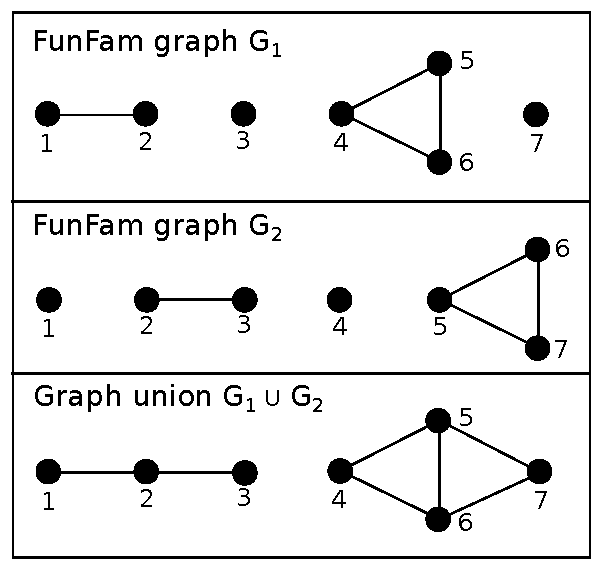
\includegraphics{./Chapter_metagenomes/fran/graph_theory}
    \caption{%
        FunFam graphs and their graph unions.
        Nodes in FunFam graphs are starting clusters that are connected by an edge if they are clustered into the same FunFam.
        FunFams are both the maximal cliques and connected components in FunFam graphs.
        Graph unions $G_u$ can be constructed from the node and edge sets of two FunFam graphs $G_1$ and $G_2$.
    }
    \label{fig:fran-graph-theory}
\end{figure}

FunFam graphs were constructed for FunFams generated by FRAN, FRAN\textsubscript{geometric} and GARDENER.
For all combinations of these graphs, a new graph $G_u = G_1 \cup G_2$ was constructed from the union of nodes and edges (\ref{fig:fran-graph-theory}).
The number of maximal cliques and connected components in $G_u$ were calculated.
If the FunFams in $G_1$ and $G_2$ agree, the number of maximal cliques and connected components will be the same.
However, if the FunFams in $G_1$ and $G_2$ partially agree, the number of connected components will decrease, whilst the number of maximal cliques will increase.
This will occur when a pair of FunFams share at least one, but not all, starting clusters.
As such, maximal cliques that were separate connected components are now connected in the same component.

\section{Results}

\subsection{Biome distribution of proteins found in metagenomes}

We assessed which biomes the metagenomic protein sequences were sampled from (\ref{fig:biome_mgnify_sequence_counts}). We used the S95 cluster representatives of MGnify's predicted protein sequences. The most populous biome is `Aquatic' with \num{142232832} sequences. This is followed by `Marine', a sub-biome of `Aquatic', with \num{104242612} sequences, which corresponds to $73.3\%$ of sequences in the `Aquatic' biome. The `Engineered' biome contains the third most sequences at \num{78057115}. Engineered biomes encompass a broad range of non-natural biomes, including industrial settings, laboratory conditions or waste treatment. Fourth is `Human' with \num{67475113} sequences, followed by the human `Digestive system' sub-biome with \num{66357615} sequences, corresponding to $98.3\%$ of sequences in `Human'. This may be caused by the large bias within metagenomics for sampling the human gut. There are no protein sequences in MGnify from the biomes `Animal' or `Soil', or any of its sub-biomes `Clay' and `Shrubland'. This is a consequence of which metagenome samples have been assembled in MGnify, for ORFs to be predicted in. Assembly is extremely expensive and slow, so is a rate-limiting factor in predicting proteins from all metagenome samples in MGnify. In the future, many more samples, from a wide assortment of biomes, will be assembled.

\begin{figure}[!hbt]
    \centering
    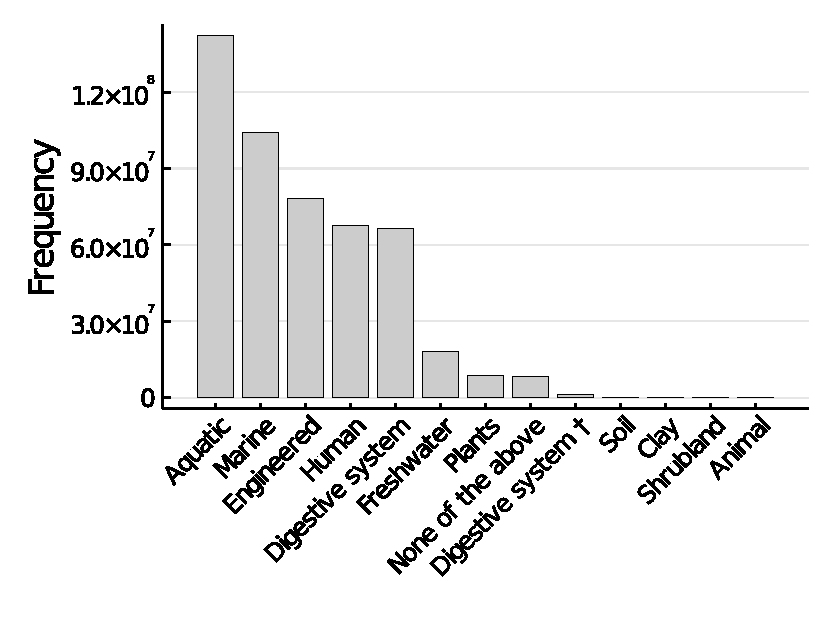
\includegraphics{./Chapter_metagenomes/biome_mgnify_sequence_counts}
    \caption{%
        Biome distribution of MGnify protein sequences.
        Biomes are ordered by number of sequences.
        † = `Host but not root:Digestive system'.
    }
    \label{fig:biome_mgnify_sequence_counts}
\end{figure}

\subsection{Metagenomes contain many α/β hydrolase domains}

We searched for α/β hydrolase domains in metagenomes using Gene$3$D and FunFams.

\subsubsection{ABH superfamily domains}

To identify CATH superfamily domains, we scanned the MGnify protein sequences against the Gene$3$D models for ABHs (superfamily ID 3.40.50.1820). To reduce the sequence redundancy of the database, we used the \num{304820129} MGnify protein sequences. We used the modified protocol to find domains in large protein sequence data sets described in \ref{sec:find_superfamily_domains_in_large_dbs}. First, the sequences were scanned against the $416$ Gene$3$D HMMs for the ABH superfamily. \num{1630166} sequences contained ABH domain hits with a significant E-value. These sequences were scanned against Gene$3$D HMMs for all superfamily domains. \num{1942889} domain hits were found for all CATH superfamilies, of which \num{1450276} were ABH domains consisting of \num{1444433} were unique ABH domain sequences. Following assignment of MDAs, \num{1435764} sequences contained ABH domains, whilst \num{194402} sequences were subsequently found to not contain ABH domains.

Prodigal was used to predict whether sequences are full-length, truncated at the N-terminus, C-terminus, or both (\ref{fig:partials}). \num{508693} proteins ($35\%$) are predicted to be full-length. $46\%$ of sequences were truncated at one end, split equally between \num{330328} N-terminal and \num{330043} C-terminal truncations. Finally, \num{266700} ($19\%$) of sequences were truncated at both ends. Due to the size of the data, we only took full-length sequences, and any ABH domains contained in full-length sequences, forward for further analysis.

\begin{figure}[!hbt]
    \centering
    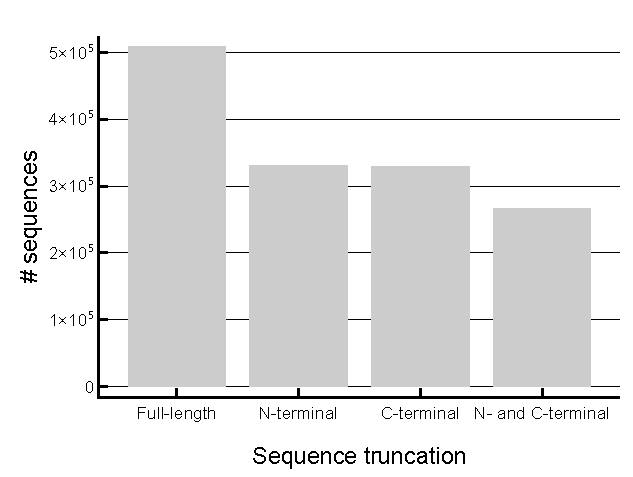
\includegraphics{./Chapter_metagenomes/sfam/partials}
    \caption{%
        Truncation of MGnify protein sequences.
        Prodigal was used to predict whether sequences are full-length, truncated at the N-terminus, C-terminus, or both.
    }
    \label{fig:partials}
\end{figure}

Lengths of ABH domains from different databases were compared. Length distribution of ABH domains from MGnify agree well with those from UniProt and Gene$3$D HMMs (\ref{fig:domain-length-distribution}). Gene$3$D ABH HMMs, built from structures in CATH v4.2, have median length $284$ residues. ABH domains in UniProt sequences from Gene$3$D have median length $259$. It is reasonable to expect that the median match length will be shorter than the median HMM length because subsequences can match HMMs with significant E-values. ABH domains in MGnify have median length $247$ residues.

\begin{figure}[!hbt]
    \centering
    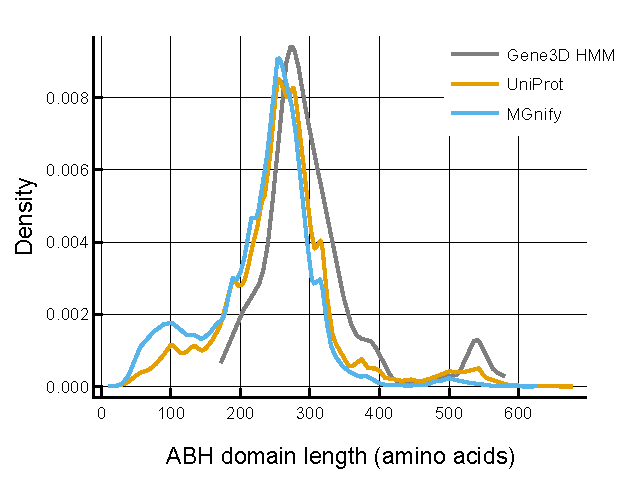
\includegraphics{./Chapter_metagenomes/sfam/domain_length_distribution_simplified}
    \caption{%
        Distribution of ABH domain lengths.
        Lengths of ABH domains from MGnify, UniProt and Gene$3$D HMMs are plotted.
        The probability density function of each distribution was estimated using kernel density estimation.
    }
    \label{fig:domain-length-distribution}
\end{figure}

\subsubsection{ABH FunFam domains}

Having found MGnify proteins that contain ABH domains, we next wanted to identify to which ABH FunFams these domains match. We scanned the full-length sequences that contain the \num{508693} ABH domains against the FunFam HMM library. Whilst CATH superfamily domains are assigned using a lenient significance threshold of E $<0.001$ in Gene$3$D, sequences are assigned to FunFams using a much stricter threshold, known as the FunFam inclusion threshold. An inclusion threshold is generated by scanning sequences from a FunFam alignment against the FunFam HMM. The lowest (worst) bit score is the inclusion threshold. There may be many and overlapping FunFam matches to a sequence. A researcher may wish to know all FunFam matches, in which case these matches are the desired output. Instead, if a researcher prefers to know an MDA, then cath-resolve-hits can be run to resolve the matches to the optimal set of non-overlapping FunFams.

After resolving FunFam MDAs, we found \num{398580} significant FunFam hits in \num{360119} sequences. Of these, there were \num{357073} hits to ABH FunFams, in \num{351853} protein sequences. There is not a one-to-one mapping between ABH hits from Gene$3$D and FunFams. Some proteins did not have any FunFams: \num{148574} proteins that were predicted to have an ABH domain do not have any hits to FunFams from any superfamily. Other proteins did not have any ABH FunFams: \num{156840} proteins that were predicted to have ABH domains do not have any hits to ABH FunFams.

Lengths of ABH FunFam matches are distributed similarly to superfamily matches (\ref{fig:sfam-funfam-match-length-distribution}). Large peaks for FunFam HMMs and FunFam matches exist at a length of 260 amino acids.

\begin{figure}[!hbt]
    \centering
    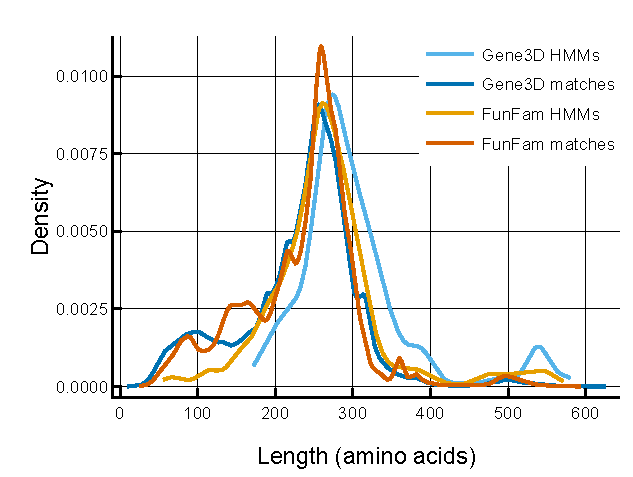
\includegraphics{./Chapter_metagenomes/funfam/sfam_funfam_match_length_distribution}
    \caption{%
        Length distribution of ABH superfamily and ABH FunFam matches.
        ABH HMMs from Gene$3$D and FunFams are also plotted.
        The probability density function of each distribution was estimated using kernel density estimation.
    }
    \label{fig:sfam-funfam-match-length-distribution}
\end{figure}

\subsection{α/β hydrolase domains are enriched in non-natural biomes}

We examined whether any biomes are enriched with ABH domains and may be promising biomes to search for candidate plastic-degrading enzymes. A linear relationship exists between the number of sequences found in a biome and the number of ABH domains found in those sequences (\ref{fig:biome_funfam_sequence_counts_scatter}). This means that ABH domains occur at a constant rate in nature. Most biomes contain the expected number of ABH domains, given the number of proteins that were found in the biome. According to a fitted regression model, `Engineered' biomes have significantly more ABH domains than expected (Fisher's $P \approx 0$). Engineered biomes encompass a broad range of non-natural biomes, including industrial settings, laboratory conditions or waste treatment. The regression model also predicts that proteins from `Human' and human `Digestive system' biomes are depleted with ABH domains (Fisher's $P \approx 0$).

\begin{figure}[!hbt]
    \centering
    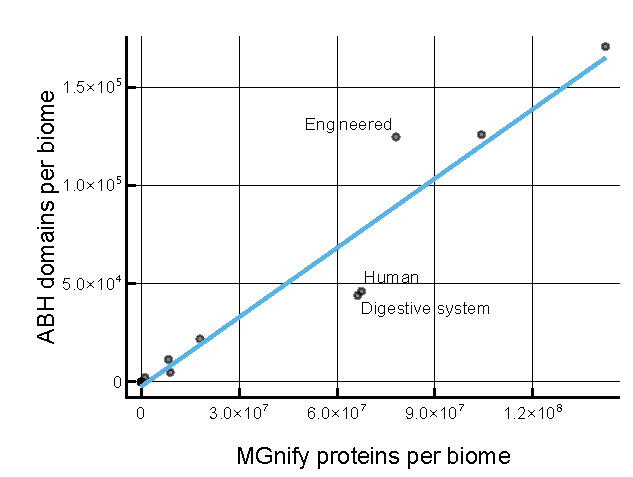
\includegraphics{./Chapter_metagenomes/funfam/biome_funfam_sequence_counts_scatter}
    \caption{%
        Relationship between the number of MGnify proteins and the number of ABH domains per biome.
        A linear regression model was fitted to the data and plotted.
        Biomes that deviate from the regression line are labelled.
    }
    \label{fig:biome_funfam_sequence_counts_scatter}
\end{figure}


\subsection{α/β hydrolase domains in metagenomes are diverse}

To understand the diversity and novelty of ABH domains in metagenomes, we clustered the \num{1065976} ABH domain sequences from MGnify (\num{508693}) and UniProt (\num{557283}) at $30\%$, $50\%$, $70\%$ and $90\%$ sequence identity. As the clustering sequence identity threshold is increased, the number of clusters increases, producing a large number of clusters at high sequence identity (\ref{fig:cath-mgy-n-clusters}). At S90, there are \num{755547} clusters, which shows that \num{319196} sequences ($30\%$) share more than $90\%$ sequence identity with another sequence in the data set. As the MGnify proteins are S90 cluster representatives, they will not cluster together at S90. Therefore, some UniProt and MGnify sequences may be clustersing into mixed origin clusters (\ref{sec:results-prok-euk}).

\begin{figure}[!hbtp]
    \centering
    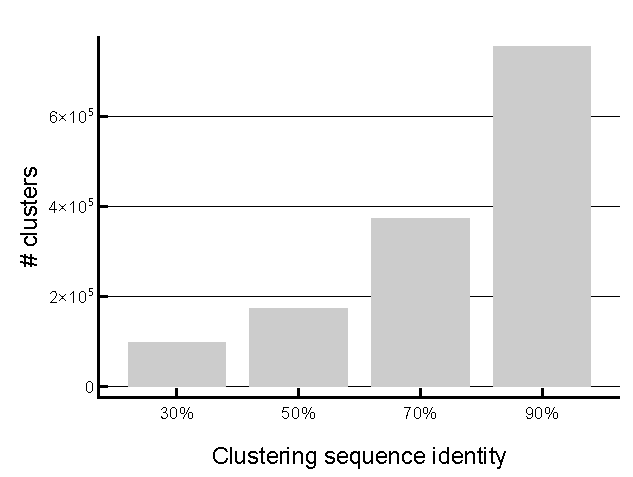
\includegraphics{{{./Chapter_metagenomes/sfam/cath_mgy_3.40.50.1820_clustering_n_clusters}}}
    \caption{%
        Number of S90 clusters in MGnify and UniProt ABH domains.
        \num{1065976} ABH domain sequences from MGnify (\num{508693}) and UniProt (\num{557283}) at $30\%$, $50\%$, $70\%$ and $90\%$ sequence identity using Linclust.
    }
    \label{fig:cath-mgy-n-clusters}
\end{figure}

As the sequence identity threshold increases, the number of singleton clusters, that contain a single sequence, increases rapidly (\ref{fig:cath-mgy-n-singletons}). \num{230666} ABH domain sequences ($21\%$) share less than $70\%$ sequence identity with all other sequences and are singletons. These singletons could represent novel functions, whose sequence diversity is not represented in gold standard databases, such as UniProt. Conventional wisdom states that protein function is conserved to approximately $60\%$ sequence identity. An analysis in 2002 found that $< 30\%$ of proteins with $> 50\%$ sequence identity have exactly the same function, according to all four digits of the EC annotation being the same \cite{Rost2002}. But hard and fast sequence identity thresholds of functional conservation for enzymes are unwise because catalysis and substrate-specificity are often determined by only a small number of residues \cite{Rentzsch2009}.

\begin{figure}[!hbtp]
    \centering
    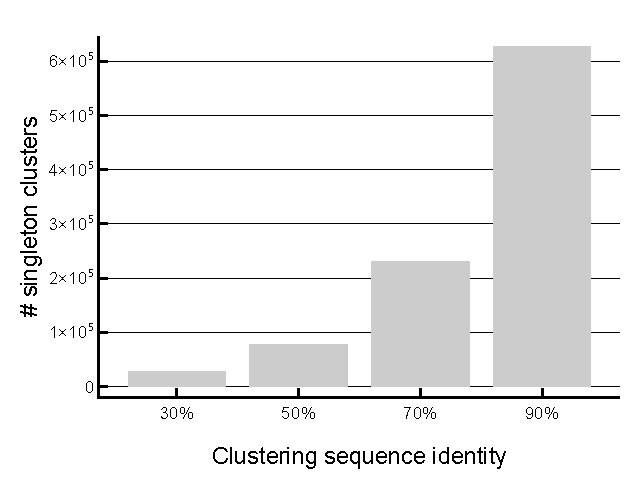
\includegraphics{{{./Chapter_metagenomes/sfam/cath_mgy_3.40.50.1820_clustering_n_singletons}}}
    \caption{%
        Number of singleton S90 clusters in MGnify and UniProt ABH domains.
        \num{1065976} ABH domain sequences from MGnify (\num{508693}) and UniProt (\num{557283}) at $30\%$, $50\%$, $70\%$ and $90\%$ sequence identity using Linclust.
    }
    \label{fig:cath-mgy-n-singletons}
\end{figure}

\subsection{α/β hydrolases in metagenomes are more similar to prokaryotic, than eukaryotic, ABH domains in UniProt}
\label{sec:results-prok-euk}

We assessed whether ABH domains from MGnify proteins are more similar to UniProt ABH domains from prokaryotes or eukaryotes. Shotgun metagenomics aims to identify all DNA from a biome. Whilst much of this genetic material will originate from prokaryotes, a significant fraction will be from eukaryotes and viruses. The question is: Are ABH domains from MGnify proteins most similar to prokaryotic or eukaryotic ABH domains in UniProt?

To answer this question, we considered mixed clusters composed of ABH domains from MGnify and UniProt. UniProt is taxonomically biased, with a prokaryotic-to-eukaryotic sequence ratio of $3:1$ ($75\%$) (\ref{fig:uniprot_sequence_taxonomy_bar} UniProt all). For proteins containing ABH domains, UniProt remains biased towards prokaryotes ($64\%$, Fisher's $P \approx 0$), but is less biased than all of UniProt (\ref{fig:uniprot_sequence_taxonomy_bar} UniProt ABH).
Mixed clusters follow a Bernoulli distribution that models the probability that a UniProt sequence is prokaryotic. The null hypothesis for mixed clusters is $B(0.64)$.

\begin{figure}[!hbt]
    \centering
    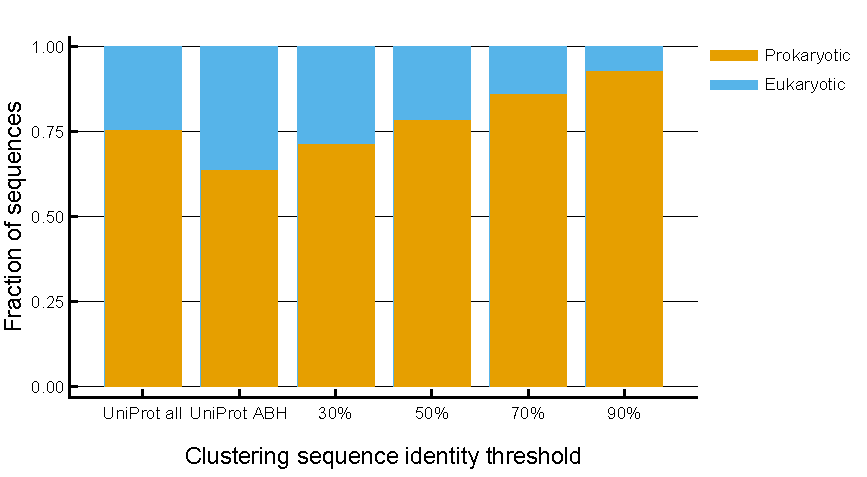
\includegraphics{./Chapter_metagenomes/sfam/uniprot_sequence_taxonomy_bar}
    \caption{%
        Assessing the similarity of MGnify ABH domains to UniProt ABH domains from prokaryotes or eukaryotes.
        \num{1065976} ABH domain sequences from MGnify (\num{508693}) and UniProt (\num{557283}) at $30\%$, $50\%$, $70\%$ and $90\%$ sequence identity using Linclust.
        Prokaryotic-to-eukaryotic ratios are plotted at each sequence identity threshold for UniProt sequences in mixed clusters.
        The prokaryotic-to-eukaryotic ratio for all UniProt sequences (UniProt all) and ABH domains in UniProt (UniProt ABH) is also plotted.
    }
    \label{fig:uniprot_sequence_taxonomy_bar}
\end{figure}

ABH domains from MGnify proteins cluster with ABH domains from UniProt, showing that metagenomes contain, at least some, previously identified sequence diversity contained in UniProt.
The prokaryotic fraction of these mixed clusters increases at higher sequence identities (\ref{fig:uniprot_sequence_taxonomy_bar}) (Fisher's $P \approx 0$ for testing all sequence identity threshold clusterings against UniProt all or UniProt ABH). There may be a number of causes for this effect, including the high fraction of non-culturable species in metagenomes, how microbiome samples are prepared before sequencing and how the protein sequences were predicted in the microbiome assemblies. These points are discussed further in (\ref{sec:discussion-prok-euk}).

We next examined the taxonomy of UniProt sequences in mixed clusters at $30\%$, $50\%$, $70\%$ and $90\%$ sequence identity. Whilst the number of mixed clusters remains stable across the sequence identity thresholds (data not shown), the prokaryotic fraction increases at higher sequence identities (\ref{fig:uniprot_sequence_taxonomy_bar}).

Many metagenomic ABHs are novel and rare, but those that are common in MGnify are also found in UniProt (\ref{fig:provenance_of_clusters_at_s70}). Most ABHs from MGnify are rare and found in small clusters with fewer than $10$ sequences. Many of the rare ABHs are also functionally novel because they are not represented in UniProt. Only $20\%$ are in mixed clusters with UniProt ABHs. On the contrary, functions of common metagenomic ABHs are already represented in UniProt. $85\%$ of clusters with $10$ or more sequences are mixed.

\begin{figure}[!hbt]
    \centering
    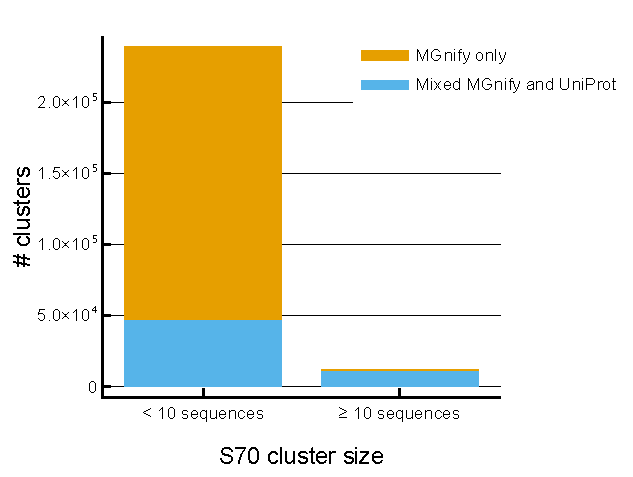
\includegraphics{./Chapter_metagenomes/sfam/provenance_of_clusters_at_s70}
    \caption{%
        Analysis of rare and common MGnify ABH domains.
        \num{1065976} ABH domain sequences from MGnify (\num{508693}) and UniProt (\num{557283}) at $70\%$ sequence identity using Linclust.
        Clusters containing MGnify sequences were grouped by size into clusters with $< 10$ sequences or $\ge 10$ sequences.
        The number of clusters is plotted grouped by whether the cluster contains `MGnify only' ABHs, or `mixed MGnify and UniProt ABHs'.
    }
    \label{fig:provenance_of_clusters_at_s70}
\end{figure}

\subsection{Little evidence for evolution of novel domains in metagenomes}

The MGnify protein sequences used in this study were sampled from biomes---and species---that have, presumably, been largely unexplored. Species in these biomes may have evolved into regions of sequence space that laboratory strains, model organisms and other well-studied species have not. These regions of sequence space may encode novel folds, domains or functions. So, have new domains evolved in metagenomes?

To answer this question, we analysed terminal regions and inter-domain sequences, i.e. contiguous regions of sequence that do not have significant matches to any Gene$3$D HMMs in MDAs (\ref{sec:intro-novel-domain}). These regions could be novel domains that have evolved in metagenomes and are, as yet, unknown. For conceptual simplicity, we considered full-length proteins whose MDAs only contain continuous domains. Therefore, single-domain proteins only have terminal sequences at each termini, whereas, multi-domain proteins can also have one inter-domain sequence between each pair of adjacent domains (\ref{sec:intro-novel-domain}).

The distribution of inter-domain sequence lengths is shown in (\ref{fig:not-matching-domains-gap-length}). The modal value is a gap length of $0$ residues, i.e. contiguous domains. Gap length probability decreases exponentially with a median of $3$ residues and a mean of $22$ residues. For comparison, CATH S95 model lengths are also plotted, which follow a positively skewed normal distribution, or log-normal distribution. The median length of these models is $145$ residues, yet $95.4\%$ of the gaps in the MGnify protein sequences are less than $145$ residues long. Furthermore, $64.8\%$ of the gaps are shorter than the shortest HMM, which is $16$ residues long.

\begin{figure}[!hbt]
    \centering
    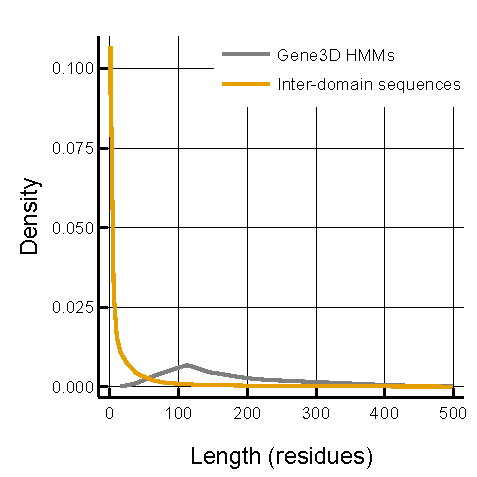
\includegraphics{./Chapter_metagenomes/sfam/inter-domain_length_dbn}
    \caption{%
        Inter-domain sequence lengths.
        The distribution of inter-domain sequences lengths that are not contained in MDAs is plotted.
        For comparison, the distribution of Gene$3$D HMM lengths is shown.
        The $x$-axis is truncated at 500 residues.
        The probability density function of each distribution was estimated using kernel density estimation.
    }
    \label{fig:not-matching-domains-gap-length}
\end{figure}

As such, terminal and inter-domain regions in metagenome proteins containing an ABH domain are unlikely to be novel domains. In order to confirm this, these sequence regions could be scanned against Pfam or PDB.

\subsection{Identification of errors in protein sequence clustering}

We noticed that some ABH domain sequences found in the MGnify proteins were not unique. Please note that the MGnify protein data set that we used in this analysis were cluster representatives. For identical domain sequences to be in different S90 clusters, the following is true: regions of sequence that flank identical ABH domains must be sufficiently different to reduce the overall sequence identity below $90\%$. We investigated these flanking regions to determine how similar the overall sequence is for proteins that contain identical ABH domains. For sequences that contain identical ABH domains, we pairwise aligned the full-length sequences using global sequence alignment with a constant gap penalty. Most pairs of sequences that have identical ABH domains are very similar across the entire sequence length (median distance $= 0.011$; \ref{fig:redundant_domain_sequences_pairwise_alignment_distance_distribution}). What's more, $61$ sequence pairs have a distance of zero. Not only are the domain sequences identical, but the entire sequences are completely identical. Finally, few sequence pairs have a distance $> 0.1$, which is approximately equal to sequence identity $< 90\%$.

\begin{figure}[!hbt]
    \centering
    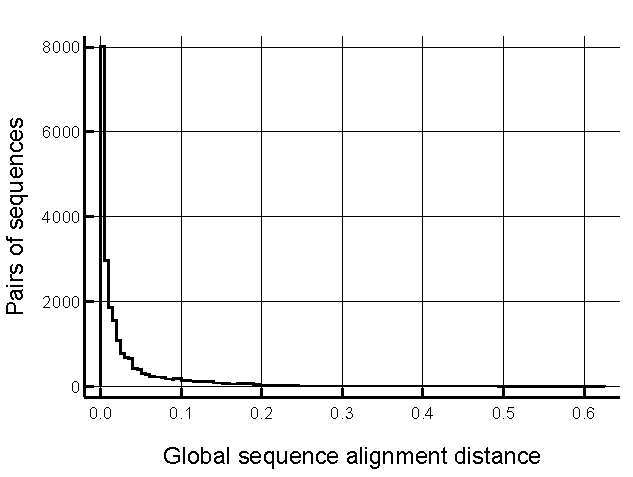
\includegraphics{./Chapter_metagenomes/sfam/redundant_domain_sequences_pairwise_alignment_distance_distribution}
    \caption{%
        Sequence alignment distances for pairs of MGnify proteins that contain identical ABH domain sequences.
        Full-length sequences were globally aligned with a constant gap penalty.
        Alignment scores were converted to distances using, $D_{S_1 S_2} = 1 - \frac{A_{S_1 S_2}}{\min(A_{S_1 S_1}, A_{S_2 S_2})}$, where $A$ is the global alignment score and $D$ is the alignment distance between two sequences $S_1$ and $S_2$.
    }
    \label{fig:redundant_domain_sequences_pairwise_alignment_distance_distribution}
\end{figure}

Whilst errors in clustering are not ideal, only \num{3676} unique domains in \num{9379} sequences are affected. We should not worry too much about this too much, as \num{9379} sequences is less than $1\%$ of the \num{508693} sequences that contain an ABH domain. But this conclusion is not satisfactory to a researcher. Why were these identical, or nearly identical, sequences not clustered together? Put simply, Linclust trades off accuracy for speed. The MMseqs2 issue tracker on GitHub (https://github.com/soedinglab/MMseqs2) has two issues, \#$88$ and \#$104$, related to identical sequences not being clustered together. The solution suggested by the developers is to increase the number of $k$-mers selected from each sequence from $21$ to $80$. Doing so will, on average, increase the number of $k$-mers that are shared between sequences and cluster centroid sequences, which will increase the probability of identical sequences ending up in the same cluster. The runtime memory requirements will quadruple from $400$ GB to $1.6$ TB. Given the current database size, this would be feasible on EBI's $1.9$ TB `big memory' machines. The sequence database need only grow by $25\%$ before this approach would no longer be tenable. To counter exploding memory requirements, MMseqs2 provides an option to load chunks of sequences into memory, at the expense of speed. We have not tested these approaches yet and debugging this workflow is tedious because it takes $\sim 24$ hours to run. But, in time, such solutions will need to be explored as the database size increases.

\subsection{α/β hydrolase domains are distributed amongst FunFams differently in MGnify and UniProt}

We explored the distribution of ABH FunFam domains in the MGnify proteins and compared it to the distribution in UniProt. CATH v4.2 has $377$ ABH FunFams. ABH domains from the MGnify proteins match $148$ of the $377$ ABH FunFams ($39\%$; \ref{fig:funfam_membership_bar_normalised_petase}) using the per FunFam inclusion thesholds.
Domains are not distributed in these $148$ FunFams the same as ABH domains in UniProt. For example, the largest FunFam in UniProt (3.40.50.1820/FF/115309) has \num{53144} members ($16\%$ of ABH domains in the $148$ FunFams), but is \nth{70} largest in MGnify with only $34$ members ($\sim 0\%$). This FunFam is associated with one molecular function: `Hydrolase activity, acting on ester bonds' (GO:0016788).
Conversely, the largest FunFam in MGnify (3.40.50.1820/FF/115552) has \num{131349} members ($37\%$) and is the fourth largest in CATH with \num{20873} members ($6\%$).
This FunFam is also associated with GO:0016788, as well as many other molecular function and biological process annotations. These include molecular functions `Chlorophyllase activity' (GO:0047746), `Pheophytinase activity' (GO:0080124) and `Bromide peroxidase activity' (GO:0019806); and biological processes `Chlorophyll metabolic process' (GO:0015994), `Response to toxic substance' (GO:0009636) and `Aromatic compound catabolic process' (GO:0019439).

\begin{figure}[!hbt]
    \centering
    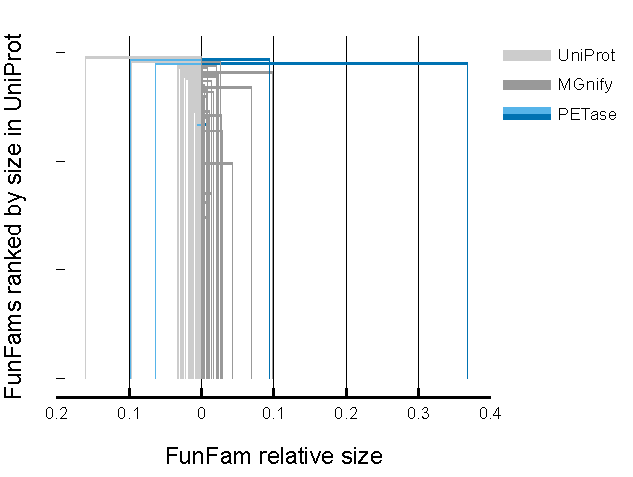
\includegraphics[width=0.9\textwidth]{./Chapter_metagenomes/funfam/funfam_membership_bar_normalised_petase}
    \caption{%
        Distribution of ABH FunFams in MGnify and UniProt.
        Of the $377$ ABH FunFams in CATH v4.2, ABH domains in the MGnify proteins match to $148$.
        These $148$ common FunFams are ranked by their size in UniProt.
        Relative size is calculated by normalising each FunFam by the total number of matches in UniProt and MGnify respectively, so that the bars on each side of the $y$ axis sum to one.
        FunFams that PETase matches to using the FunFam inclusion threshold are highlighted in blue.
    }
    \label{fig:funfam_membership_bar_normalised_petase}
\end{figure}

PETase matches to three ABH FunFams (3.40.50.1820/FF/115552, 3.40.50.1820/FF/115534 and 3.40.50.1820/FF/115660) that are associated with functions that are similar to hydrolytic depolymerisation of PET. The largest FunFam for the MGnify proteins, 3.40.50.1820/FF/115552, was discussed in the previous paragraph. PET is a polymer of ethylene terephthalate, an aromatic monomer, which is similar to large, complex organic molecules, such as chrlorophyll, pheophytin and steroid hormones. $37\%$ of MGnify ABH domains are in this FunFam. The second largest FunFam, 3.40.50.1820/FF/115534, contains $9\%$ of MGnify ABH domains, which corresponds to the $10\%$ of UniProt ABH domains in this family. This FunFam is associated with $19$ molecular function, and $32$ biological process, GO terms related to lipid hydrolysis, signalling and inflammatory responses. The smallest FunFam, 3.40.50.1820/FF/115660, is proportionally $1.8$ times larger than in UniProt. This FunFam is associated with $19$ molecular function, and $24$ biological process, GO terms related to lipid hydrolysis and steroid hormone signalling. Chemically and structurally, PET resembles lipids, which are polymers of organic monomers.

\subsection{Generating FunFams at gigascale}

\begin{itemize}
    \item Harry Scholes designed the FRAN and FRAN\textsubscript{geometric} algorithms.
    \item Clemens Rauer implemented the algorithms and ran the benchmarks.
    \item Harry Scholes analysed and interpreted the benchmarking results.
\end{itemize}

Sequence databases are growing rapidly in size and diversity, which, in turn, benefits the quality of FunFams. Can our methods cope with billions of sequences at gigascale? Here, we benchmark two new algorithms, FRAN and FRAN\textsubscript{geometric}, to generate FunFams on arbitrarily large numbers of sequences (\ref{methods:fran}).

% and kinases
We tested the performance of FRAN and FRAN\textsubscript{geometric}, considering the quality of the resulting FunFams. For comparison, we benchmarked against GARDENER, the gold standard method to generate FunFams.
We tested these three approaches on α/β hydrolases (\ref{tab:fran}).
All three methods generate a similar number of FunFams, with a similar number of FunFams having EC terms.
FRAN ($1048$) and FRAN\textsubscript{geometric} ($1042$) generate very similar numbers of FunFams.
Clusterings are very similar to GARDENER, as measured by the Rand index, for FRAN ($0.87$) and FRAN\textsubscript{geometric} ($0.88$). FRAN and FRAN\textsubscript{geometric} form almost identical clusters, as measured by the Rand index of $0.95$.

\begin{table}[hbt!]
    \centering
    \caption{%
        FunFams generated by FRAN, FRAN\textsubscript{geometric} and GARDENER.
        FunFams were generated for the α/β hydrolase family,
        CATH superfamily 3.40.50.1820.
        The number of starting clusters, FunFams, FunFams with EC terms and
        the Rand index of FunFam agreement with GARDENER are reported.
    }
    \label{tab:fran}
    \begin{tabular}{lcccc}
        \toprule
        \textbf{Method} & \textbf{Starting clusters} & \textbf{FunFams} & \textbf{FunFams with EC} & \textbf{Rand index} \\
        \midrule
        GARDENER & $1546$ & $1188$ & $298$ & $1.00$ \\
        FRAN & $1546$ & $1048$ & $255$ & $0.87$ \\
        FRAN\textsubscript{geometric} & $1546$ & $1042$ & $274$ & $0.88$ \\
        \bottomrule
    \end{tabular}
\end{table}

We confirmed that FRAN and FRAN\textsubscript{geometric} parition starting clusters into similar FunFams by constructing graphs of FunFams and calculating graph theoretic measures on them (\ref{fig:fran-graph}).
FRAN, FRAN\textsubscript{geometric} and GARDENER have as many maximal cliques as connected components because FunFams are hard clusters.
FunFam clustering by FRAN and FRAN\textsubscript{geometric} have very similar global agreement, as shown by
the graph union of GARDENER and FRAN (G $\cup$ F) having approximately the same number of connected components and maximal cliques as the graph union of GARDENER and FRAN\textsubscript{geometric} (G $\cup$ Fg).
Both graph unions are below the $y = x$ line, which shows that they have fewer connected components than maximal cliques.
This means that FRAN and FRAN\textsubscript{geometric} generate different FunFams to GARDENER, but that these FunFams form larger connected components, comprised of multiple maximal cliques, in the graph union because some starting clusters are shared between the FunFams.
This is confirmed by the graph union of FRAN and FRAN\textsubscript{geometric} (F $\cup$ Fg), which has fewer connected components than maximal cliques, showing that many of the FunFams generated by these two methods intersect.
Finally, the graph union of all three methods (G $\cup$ F $\cup$ Fg) has slightly fewer cliques than G $\cup$ F, or G $\cup$ Fg, but far fewer connected components.
More FunFams are being merged into the same connected components in (G $\cup$ F $\cup$ Fg) because FRAN and FRAN\textsubscript{geometric} parition the starting clusters into different FunFams.
However, these FunFams intersect with other FunFams generated by the other method and by GARDENER.
Whilst FunFams generated by FRAN and FRAN\textsubscript{geometric} do not agree perfectly with GARDENER, the FunFams are similar, as shown by the large number of FunFams that have intersecting starting clusters.
Overall, the FRAN and FRAN\textsubscript{geometric} algorithms produce sufficiently similar FunFams to be taken forward for further analysis.

\begin{figure}[!hbt]
    \centering
    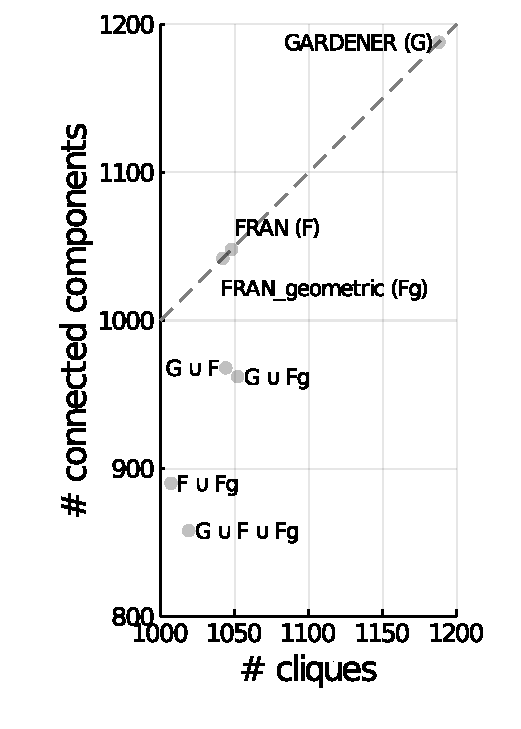
\includegraphics{./Chapter_metagenomes/fran/graph_union_cliques_connected_components_scatter}
    \caption{%
        FunFam graph theoretic benchmarks for FRAN (F), FRAN\textsubscript{geometric} (Fg) and GARDENER (G).
        Graphs were constructed for FunFams that are composed of $> 1$ starting cluster.
        Perfect FunFam clustering is shown as a dotted line at $y = x$.
        $\cup$ denotes the graph union operation.
    }
    \label{fig:fran-graph}
\end{figure}

The EC purity of FunFams generated by FRAN and FRAN\textsubscript{geometric} were similar to GARDENER (\ref{fig:fran-ec}).
There was no significant difference between the EC purity distribution for FunFams produced by GARDENER and FRAN (two-sided Mann-Whitney $P = 0.72$), or GARDENER and FRAN\textsubscript{geometric} (two-sided Mann-Whitney $P = 0.85$).
Therefore, the functional purity of FunFams generated by FRAN and FRAN\textsubscript{geometric} were comparable to FunFams generated by GARDENER.

\begin{figure}[!hbt]
    \centering
    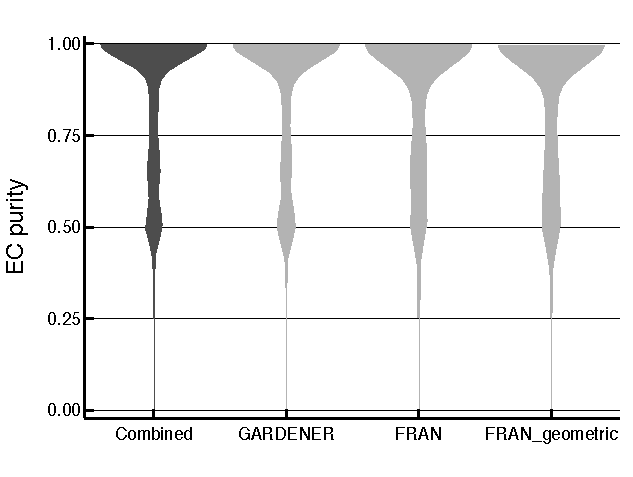
\includegraphics{./Chapter_metagenomes/fran/funfam_ec_purity}
    \caption{%
        FunFam EC purity benchmarks for FRAN, FRAN\textsubscript{geometric} and GARDENER.
    }
    \label{fig:fran-ec}
\end{figure}

As FRAN and FRAN\textsubscript{geometric} produce very similar FunFams, but FRAN\textsubscript{geometric} is more computationally expensive, FRAN will be taken forward to be used to generate FunFams of large CATH superfamilies.

\section{Discussion}

\subsection{A large number of α/β hydrolase domains were found in metagenomes}

Whilst MGnify contains many analyses of metagenomic sequencing studies (\num{315181} as of April 14, 2020), only a small subset ($6\%$) of studies have so far been assembled (\num{18291} as of April 14, 2020). The number of protein sequences identified in each biome probably does not reflect the sequence and functional diversity of the biome (\ref{fig:biome_mgnify_sequence_counts}). Rather, the number of sequences reflects the degree to which each biome has been sampled, which samples have been assembled, or which assemblies have had ORFs predicted. For example, there have been vast metagenomics projects of marine \cite{Sunagawa2015} and human gut \cite{Almeida2019,Forster2019} microbiomes that will have captured the sequence diversity in these biomes. Comparatively, plants, soil and other animal biomes have been neglected.

The modified protocol that we used to find superfamily domains in large sequence data sets (\ref{sec:find_superfamily_domains_in_large_dbs}) saved vast computational resources. Scanning $10^6$ sequences MGnify proteins against the $416$ ABH Gene$3$D HMMs took approximately $30$ minutes on four cores---that is, $3.6$ CPU weeks in total. Scanning $10^4$ sequences against all Gene$3$D HMMs took approximately $60$ minutes on four cores---that is, $3.9$ CPU weeks for all \num{1630166} sequences that had a significant ABH hit.
Using these timings, we can estimate that searching all of the MGnify proteins against all Gene$3$D HMMs would take $14$ CPU years, whilst searching the redundant database of $1.1$ billion sequences would take $50$ CPU years. Additionally, by implementing this pipeline in Nextflow, we could conveniently split up the sequence data sets into managable chunks, that could be processed in an embarrassingly parallel way, by many independent jobs, each with low memory and CPU requirements.

We identified a large number of diverse ABH domain sequences from full-length and truncated ORFs (\ref{fig:partials}). It is reasonable to assume that sequences truncated at one terminus would, on average, be longer than sequences truncated at both termini. However, the median length of sequences truncated at either terminus is 136 residues, whereas, sequences truncated at both termini have median length $164$ residues. This could have been caused by the Prodigal algorithm \cite{Hyatt2010}. Prodigal looks for ribosome binding sequence motifs, such as the Shine-Dalgarno sequence, and an in-frame stop codon to predict proteins from ORFs. To reduce the number of false positive ORFs, Prodigal penalises sequences shorter than $250$ bp by a linear factor that is proportional to their length \cite{Hyatt2010}. These features are strong, so short sequences that are truncated at one end can still end up with favourable scores. However, sequences that are truncated at both ends must be long to have favourable scores.

Because we identified a large number of ABH domains, we took full-length sequences, and any ABH domains contained in full-length sequences, forward for further analysis. ABH domains identified in the MGnify proteins follow the same length distribution as known ABH domains from UniProt (\ref{fig:domain-length-distribution}). This finding indicates the quality of MGnify data. Firstly, it suggests that the MGnify assemblies represent real contigs found in microbiomes. Secondly, and \emph{propter hoc}, the predicted ORFs and protein sequences real.

$70\%$ of ABH domains in MGnify, predicted by Gene$3$D, were assigned to an existing ABH FunFam using the strict per FunFam inclusion threshold (\ref{fig:sfam-funfam-match-length-distribution}). There are a number of possible causes for this. Firstly, new functions could have evolved in metagenomes. These functions would not be present in UniProt. Because FunFams are generated using sequences from UniProt, FunFams will not be generated that represent these newly-evolved functions. Secondly, FunFams are generated from starting clusters that are associated with an experimentally characterised function. ABHs with novel and uncharacterised functions will not be covered by FunFams.

It is encouraging that ABH domains were found in engineered biomes more frequently than the background rate for MGnify proteins (\ref{fig:biome_funfam_sequence_counts_scatter}). This finding may represent an increased potential to find proteins with biotechnology applications similar to PETase, which was found in an engineered environment \cite{Yoshida2016}. Conversely, ABH domains were depleted in the human digestive system (\ref{fig:biome_funfam_sequence_counts_scatter}). Whilst α/β hydrolase proteins are present in the digestive system to degrade proteins and lipids, the diversity of these proteins may not be that high. Considering that the MGnify proteins are cluster representatives, the importance (concentration) of these enzymes may be obscured by the lack of sequence diversity.

\subsection{α/β hydrolase domains in metagenomes are diverse}

To understand their diversity and novelty, ABH domains from MGnify proteins were clustered with ABH domains from UniProt proteins. A large number of clusters (\ref{fig:cath-mgy-n-clusters}) and singleton clusters (\ref{fig:cath-mgy-n-singletons}) result at high sequence identity. This demonstrates that the ABH domain fold can accommodate a high diversity of sequences, whilst leaving the structure intact. Evidently, this robustness has been exploited by evolution to produce a wide variety of ABH domain functions.

Sequences clustered together, as shown by the number of clusters always being much lower than the number of sequences. The MGnify proteins are S90 cluster representatives. So this result suggests that some of the MGnify ABH domain sequences are clustering with those from UniProt. It should be noted that the domain sequences from UniProt have not been filtered to remove redundant sequences, however, it is unlikely that only the UniProt sequences clustered together. If MGnify and UniProt ABH domains clustered together, this would further increase our confidence in the quality of the assemblies and ORFs in MGnify.

It is remarkable that $21\%$ of ABH domain sequences are singletons at S70. This means that, whilst the overall chemistry of the catalysis may be the same, these sequences are likely to have different (specific) functions, or be regulated differently. Additionally, the large number of singletons at S70 suggests that biomes have not been sampled exhaustively. Many more functions are out there waiting to be discovered. As more biomes are studied and more samples are collected, I expect the number of clusters and singletons to continue to increase.

Given both of these findings, it appears that clustering at S70 or S90 is too stringent for the degree of sequence diversity in a superfamily and clustering at S60 is more likely to obtain meaningful clusters. Clustering at this level makes sense because protein function is conserved to approximately $60\%$ sequence identity \cite{Rost2002,Rentzsch2009}. Whilst this sequence identity threshold may be true for ABH domains, it may not be true for the other CATH superfamilies.

\subsection{α/β hydrolases in metagenomes are more similar to prokaryotic, than eukaryotic, ABH domains in UniProt}
\label{sec:discussion-prok-euk}

UniProt is biased towards prokaryotes, but this bias is less so in proteins that contain ABH domains (\ref{fig:uniprot_sequence_taxonomy_bar}). We used the taxonomic bias for proteins containing ABH domains to define a null distribution for mixed clusters. Other biases may affect the taxonomic distribution of proteins in MGnify, for example which biomes were sampled, how high the coverage of sampling was, how samples were prepared prior to sequencing, which samples were assembled, and choice of gene callers. Despite these biases, we can arguably be more confident about mixed, rather than single origin, clusters because these sequences are present (independently) in both MGnify and UniProt.

We observed that the prokaryotic fraction of mixed clusters increases at higher sequence identities (\ref{fig:uniprot_sequence_taxonomy_bar}). There may be a number of causes for this effect. Firstly, UniProt may not contain representatives of eukaryotic ABH domains found in metagenomes. Metagenomes contain a large number of unknown species that cannot yet be cultured. It has been estimated that only $1\%$ of microorganisms have been cultured \cite{Rinke2013}. Many of these species are likely to be eukaryotic \cite{Saary2019}, whether small or single-celled. It is reasonable to assume that ABH domains have evolved in these species to allow them to occupy particular niches. Therefore, it is likely that these domain sequences will not be present in UniProt. Secondly, metagenomic samples are size fractionated to remove larger objects in samples, so eukaryotes are more likely to be removed and prokaryotes are more likely to be retained. Thirdly, MGnify only uses prokaryotic gene callers to predict ORFs in assemblies (\ref{sec:mgnify-methods}). Prokaryotic gene callers may have a high false negative rate on eukaryotic contigs. Eukaryotic gene callers, such as GeneMark-EP \cite{Bruna2020}, MetaEuk \cite{LevyKarin2020}, or EuGene \cite{Sallet2019}, could be applied in parallel with the current prokaryotic gene callers. These three factors will contribute to eukaryotic proteins being underrepresented in the MGnify proteins. This analysis should be repeated when MGnify incorporates eukaryotic gene calling into its protein prediction pipeline.

Overall, presence of mixed clusters shows that ABH domains in metagenomes are not distinct from previously known sequences in UniProt. Rather, we see sequence conservation alongside evolution of new functions. New functions are generated by exploration of previously unexplored regions of sequence space to enable organisms to survive and occupy different niches. Retention of function by an organism is a fitness cost: if functions are not required, they will be lost. Conservation of previously-known functions demonstrates that these functions are required by species to survive in particular biomes

\subsection{Little evidence for the evolution of novel domains in metagenomes}

We assessed whether novel domains had evolved in metagenomes (\ref{fig:not-matching-domains-gap-length}), but found little evidence for it. Inter-domain lengths were short, so the vast majority of metagenomic protein sequence is covered by a significant Gene$3$D hit to a CATH superfamily. Therefore, it appears that novel domains have not evolved in metagenomes. There are, however, some caveats to this conclusion. Although we have little evidence of novel domain evolution in proteins containing ABH domains, we cannot extrapolate these conclusions to metagenomic protein sequences in general. Similar analyses on different superfamilies, subsets of superfamilies, or all superfamilies would be required before drawing general conclusions about metagenomes. Further caution should be exercised because $91\%$ of sequences containing ABH domains in Pfam are single-domain proteins (\num{73297} out of \num{80360} sequences in Pfam family PF00561), which only have two terminal regions and no inter-domain regions.

\subsection{α/β hydrolase domains are distributed amongst FunFams differently in MGnify and UniProt}

As FunFams are functionally pure, functions of proteins can be predicted by mapping domains to FunFams. The ABH domain from PETase was mapped to three FunFams involved in the hydrolysis of large organic biomolecules (\ref{fig:funfam_membership_bar_normalised_petase}). PET is a polymer of ethylene terephthalate, a monomer composed of an aromatic ring with carboxy groups at the 1 and 4 ring positions. A carboxy group at the 1 position of one monomer reacts with a second monomer's ethanol moiety attached to the single-bonded oxygen of the carboxy group at the 4 position. PET resembles the substrates of proteins that map to the same FunFams. Lipids are carbon polymers. Many plastics, including PET, are polyesters, i.e. polymers formed by esterification between carboxylic acids and alcohols of monomers. Chrlorophyll, pheophytin and steroid hormones are composed of many aromatic groups. These findings naturally give rise to a hypothesis for the origins of PETase. A hydrolase, whose cognate ligand is some type of large organic biomolecule, evolved to degrade PET under massive selection pressures.

In addition, MGnify ABH domains were mapped to FunFams (\ref{fig:funfam_membership_bar_normalised_petase}). One possible reason for finding so few matches in MGnify to the largest ABH FunFam in UniProt (3.40.50.1820/FF/115309) could be that the FunFam is large and so the sequence alignment might be poor. $16\%$ of UniProt ABH domains are in this family. Thus, the resulting HMM would not be very informative, so few sequences would have high-scoring matches. Low-scoring matches would be trumped by higher-scoring matches when the MDAs were resolved. 3.40.50.1820/FF/115552 contains $37\%$ of MGnify ABH domains. Compared with UniProt, this family is significantly expanded in metagenomes, which suggests that this FunFam increases the fitness on species living in diverse microbiomes. This family is associated with hydrolysis of ester bonds and large biomolecules. This might mean that hydrolases have evolved to metabolise other synthetic man-made materials, such as other types of plastics. These materials are certainly in the environment, so there is a selection pressure for organisms to make use of these energy sources. If so, it is likely that the ABH domain will evolve to degrade these materials because of its incredible functional plasticity.

% Moved to final chapter
% \subsection{Targeted assembly of metagenomes and functional validation}
%
% 6\% of microbiome samples in MGnify have been assembled, which is just the tip of the iceberg. A mountain of information remains to be mined. Going forward, we will perform targeted assembly of samples from particular biomes \ref{fig:biome_funfam_sequence_counts_scatter}. We will choose samples from biomes that look promising for finding plastic-degrading enzymes, whether that be from biomes that: contain more ABH domains than expected by chance, contain proteins with high sequence identity to PETase, or from manual examination of biomes by curators. We only plotted high-level biomes that do not convey very specific information about the environments that samples were collected from (\ref{sec:mgnify-methods}) in \ref{fig:biome_funfam_sequence_counts_scatter}. But when selecting samples to be assembled, we will consider more specific biome assignments that are lower in the GOLD biome ontology \cite{Mukherjee2019}. We will predict proteins from the assembled contigs, which will be analysed for their similarity to PETase and their plastic-degrading potential.
%
% We hope that this iterative pipeline will produce a wealth of information that can be analysed to discover new plastic-degrading enzymes in nature. Putative sequences will be functionally validated using picodroplet functional metagenomics \cite{Colin2015} in a collaboration with Florian Hollfelder at Cambridge. We will be able to validate between 10 and 100 sequences using this method. Alongside true positives for positive controls, we will introduce mutations into PETase at key sites. These mutations may change the efficiency of PET degradation, or even change the function or substrate-specificity to another plastic. Furthermore, we will test putative sequences that we discover through analyses similar to those performed in this work.

\subsection{The FRAN algorithm allows FunFams to be generated at gigascale}

Presently, we are facing challenges generating FunFams of large superfamilies using GARDENER because all starting clusters are required to be kept in memory as the GeMMA tree is grown. Our current workaround is to run large superfamilies on a high-memory machine with $3$ TB memory, but we are already approaching the memory limit of these machines. Memory is expensive and 3 TB is already a lot of memory, so we need to develop a low-memory strategy that will allow FunFams to be scaled to extremely large superfamilies in the future. Whole-genome sequencing and metagenomics are now possible, are being adopted and are growing in popularity. As such, a scalable protocol would allow FunFams to be generated using protein sequences from metagenomes and from UniProt. Also, we currently only generate FunFams from S90 clusters that have at least one experimental GO term annotation. A scalable protocol will allow us to remove this restriction.

The current restriction means that every FunFam is associated with a known function, which is useful for function prediction.
However, this means that FunFams cannot be generated for proteins with novel functions.
If a FunFam has no annotated functions, putative functions could be predicted by transferring any functions from the nearest $k$ neighbouring FunFams, within some E-value radius $r$.
Neighbouring FunFams can be found by pairwise HMM alignment to all other FunFams in the same superfamily.
These putative functions will be useful to experimentalists to guide their choice of proteins to validate, which will be particularly important when validating proteins with novel functions from metagenomes.
Alternatively, FunFams can be annotated \emph{post hoc}, whenever one of the members has been experimentally characterised.
We hypothesise that the number of FunFams will increase dramatically to reflect the increase in sequence and functional diversity present in these additional sequences.

Here, we designed two divide-and-conquer algorithms, FRAN and FRAN\textsubscript{geometric}, to generate FunFams on subsets of a superfamily's sequences at a time. The algorithms first sample starting clusters into different groups, which are used as independent inputs to GeMMA and FunFHMMer. The FunFHMMer outputs are then pooled and treated as starting clusters for a second round of GeMMA and FunFHMMer, which allows sequences that were sampled into different groups to be merged into the same FunFams. Curiously, we observed no difference between the quality of FunFams that FRAN, FRAN\textsubscript{geometric} and GARDENER generated (\ref{fig:fran-graph,fig:fran-ec}).

Originally, we hypothesised that if a superfamily's sequences were subset into different groups, each group should---as far as possible---retain the same characteristics as all of the sequences combined. Comparing the performance of FRAN to FRAN\textsubscript{geometric} shows that uniform random sampling produces as good FunFams to the geometric sampling strategy, employed to respect the evolutionary relationships between sequences. This result demonstrates the power of GARDENER at being able to fix any clustering errors in the first round of FunFamming with a second round.

FRAN\textsubscript{geometric} is more expensive than the null model because it requires two clustering steps at S90 and S30, as well as drawing two random numbers when sampling each starting cluster into groups---one random number to sample an S30 and one random number to sample an S90 contained therein. Conversely, FRAN requires one clustering step at S90, followed by one random number to sample each starting cluster. Going forward, FRAN will need to be benchmarked on more superfamilies and compared to GARDENER. If the performance is comparable across many superfamilies, then FRAN should be used to generate FunFams of problematically large superfamilies, whilst vanilla GARDENER could be used on manageable superfamilies.

\subsection{Conclusion}

This work laid the foundations for two exciting new avenues of research. First, we conducted a proof-of-concept study into mining very large protein sequence data sets for novel functions. We used our tools---CATH, Gene$3$D and FunFams---to search metagenomes for plastic-degrading enzymes similar to PETase. Sequence databases are continue to grow in size, so following on from this, we investigated approaches that would allow FunFams to be generated on an arbitrarily large number of sequences. We decomposed the FunFam generation algorithm, GARDENER, using a divide-and-conquer random sampling approach, FRAN. This approach will allow FunFams to be generated on ever-growing sequence databases, including metagenomes, future-proofing FunFams for many years to come.

% \references
